\label{sec:vbf-bdt}
The BDT is trained with scikit-learn package~\cite{scikit-learn}.
The classifier has 200 trees and employs the AdaBoost method.
The background sample is taken from data events with $80~\GeV < \Mbb <100$~\GeV~
and $150~\GeV<\Mbb<190$~\GeV~and contains approximately 690k events for
the \fourcentral channel and 90k events for the \twocentral channel.
The signal contamination in this region is negligible.
The $Z$ contribution to the low-mass sideband is not explicitly accounted
for due to its small size (see Tables~\ref{tab:cutflow_4cen}
and~\ref{tab:cutflow_2cen} for the number of events of each type passing pre-selection).
As will be shown in Figure~\ref{fig:vbf-BDTResponse},
the BDT response of the QCD-produced \zjets~ sample is very similar to the background samples. 

The signal sample is the VBF Monte Carlo simulated dataset and
contains 10k events for the \fourcentral channel and 2k events for
the \twocentral channel.  Half of the signal and background samples are
used for training and the other half are used for validation.

The following variables are used for training:
\begin{enumerate}
\item $M_{\rm JJ}$, the invariant mass of the VBF jet pair. 
\item $p_{\rm T,JJ}$, the transverse momentum of the VBF jet pair. 
\item $\cos{\theta}$, cosine of the polar angle of the cross product of the momenta of the VBF jets in the Higgs boson's rest frame.
\item $Max (\eta)$, the maximum between the absolute values of the pseudo-rapidity of the VBF jets: $Max (\eta) \equiv max( |\eta_{J1}|, |\eta_{J2}| )$
\item $\eta* = \frac{1}{2}( |\eta_{\rm J1}| + |\eta_{\rm J2}| - |\eta_{\rm B1}| - |\eta_{\rm B2}|)$, average pseudo-rapidity difference between VBF and signal jets.
\item $min\Delta R$(J1), minimum angular separation between the leading VBF jet and its closest jet. 
\item $min\Delta R$(J2), minimum angular separation between the sub-leading VBF jet and its closest jet. 
\item QGTagger(J1),  the number of tracks associated to the leading VBF jet, as described in Section~\ref{sec:vbf-qgtagging}.
\item QGTagger(J2),  the number of tracks associated to the sub-leading VBF jet, as described in Section~\ref{sec:vbf-qgtagging}.
\item $p_{T}$ balance, the ratio of vectorial and scalar sum of signal and VBF jets \pT,  $\frac{\overrightarrow{p_{T}}(J1)+\overrightarrow{p_{T}}(J2)+\overrightarrow{p_{T}}(B1)+\overrightarrow{p_{T}}(B2) }{ p_{T}(J1)+p_{T}(J2)+p_{T}(B1)+p_{T}(B2)}$
\item $\Delta M_{\rm JJ}$, the difference between largest invariant mass calculated using all jet pairs and only VBF jet pair. 
\end{enumerate}

The distributions of all input variables for each channel are
shown in Figures~\ref{fig:vbf-BDTInputs2cen} and Figures~\ref{fig:vbf-BDTInputs4cen}.
As shown in Figure~\ref{fig:vbf-BDTInputsCor}, most variables have a
small correlation factor of less than 0.1 with \Mbb.
The most correlated variables with \Mbb is $\Delta M_{\rm JJ}$.
Further studies of the correlation with \Mbb and the BDT variables,
the relative importance of each variable in the BDT, and a 3-fold
validation test are shown in Appendix~\ref{sec:vbf-app-bdt}.
From these studies we conclude that the BDT discriminant is not
significantly correlated with \Mbb with the exception of very high BDT scores.

The BDT response for  the signal and background training and validation
samples for both channels is shown in Figure~\ref{fig:vbf-BDTResponse}.
In the \fourcentral channel the VBF \Hbb BDT distribution peaks at 0.03.
The background sample peaks at -0.02.  In the \twocentral channel the
VBF \Hbb distribution has a single broad peak at 0.05 and the
background peaks at -0.02. Good agreement is seen between the training
and validation datasets, indicating that the BDT training is adequate.
A Kolmogorov-Smirnov test is used to check the compatibility between
the training and validation datasets.  The \twocentral channel has
a 0.52 $p$-value for the observed agreement in the background sample
and 0.58 $p$-value for the signal sample. The \fourcentral channel has
a $p$-value of 0.95 for the background and $p$-value of 0.99 for the signal.
Figure~\ref{fig:vbf-BDTResponse} also shows the compatibility of the BDT
shapes for all samples considered in this analysis.
TheggF Higgs production and QCD-produced \zjets ~ samples have a
nearly identical response to the background sample in the \fourcentral channel.
In the \twocentral channel these samples have a slightly higher average BDT score than the background distribution.
The EWK \zjets ~ production has a most probable BDT score which is higher than the
background samples, but less than the VBF \Hbb sample in both cases. 

For the \twocentral channel, we choose a region in which
a sufficiently large number of \zjets{} events pass the BDT to
adequately control the contribution of this background in the final fit.
The top 80\% of the VBF signal events pass this requirement to define the first signal region.
The second encompasses the remainder of the BDT distribution.


This definition of the regions is a conservative approach that ensures a constraining power of the \zjets{} contribution sufficient to prevent biasing the Higgs strength (see Section~\ref{sec:vbf-ztreat} and Appendix~\ref{sec:vbf-app-alternative2cen} for more details). 
Alternative definitions of the SRs, aimed at maximizing the sensitivity for the Higgs boson, 
have been considered and discarded in favor of having higher precision in determining the \zjets{} contribution in each region.
Table~\ref{tab:BDTSensitivity} illustrates the impact of the choice of SR I definition on the overall Higgs sensitivity and 
the precision on the \zjets{} contribution in that region.
For example, extending the lower boundary of the SR I from including 50\% to 80\% VBF events, 
the \zjets{} contribution grows by a factor of five, corresponding to a 2.7 times improvement in constraining power, while the Higgs sensitivity is reduced by 17\%.   The last column of Table~\ref{tab:BDTSensitivity} is chosen as the BDT region definition. 

For the \fourcentral channel, we scan the VBF signal events in the entire BDT scores to maximize the sum of $\frac{S}{\sqrt{B}}$ for the top 70\% VBF signal to define in total four signal regions. In this channel, the \zjets{} contribution is larger and the constraining power in each SR is adequate to prevent large bias to the Higgs strength (see Section~\ref{sec:vbf-zunblind}).
Therefore the ad-hoc adjustment of the SR boundaries adopted for \twocentral is not necessary.

The definition of the signal regions, the yields of each processes and the estimation of sensitivity are listed in Tables~\ref{tab:BDTReg2cen_alt} and ~\ref{tab:BDTReg4cen_alt}. 


\begin{table}[]
\centering
\caption{Higgs and \zjets{} sensitivity for different definitions of BDT regions in \twocentral channel. The $\Delta \mu_H$ is estimated with Asimov fit for all regions and channels combined. The $\Delta \mu_Z$ is estimated in sideband only fit for SR I of the \twocentral channel. The most sensitive region is always defined to retian VBF events with top x\% BDT scores. The rest of the regions are defined to maximize the sum of $\frac{S}{\sqrt{B}}$. The final configuration we choose is the last column such that we have sufficient constraining power of \zjets{}.}
\label{tab:BDTSensitivity}
\resizebox{\textwidth}{!}{
\begin{tabular}{|c|c|c|c|c|c|}
\hline
                                                                                             & \begin{tabular}[c]{@{}c@{}}4 regions\\     SR I top 30\% VBF\end{tabular} & \begin{tabular}[c]{@{}c@{}}3 regions\\   SR I top 50\% VBF\end{tabular} & \begin{tabular}[c]{@{}c@{}}3 regions\\   SR I top 60\% VBF\end{tabular} & \begin{tabular}[c]{@{}c@{}}3 regions\\   SR I top 70\% VBF\end{tabular} & \begin{tabular}[c]{@{}c@{}}2 regions\\   SR I top 80\% VBF\end{tabular} \\ \hline
$\Delta \mu_H$                                                                               & 1.4                                                                       & 1.67                                                                    & 1.71                                                                    & 1.78                                                                    & 1.84                                                                    \\ \hline
\begin{tabular}[c]{@{}c@{}}$\Delta \mu_Z$\\ 2 central SR I\\ Sideband only fit\end{tabular}  & 5.0                                                                       & 3.37                                                                    & 2.6                                                                     & 1.6                                                                     & 1.25                                                                    \\ \hline
\begin{tabular}[c]{@{}c@{}}\# Z events in \\ the side band of \\ 2 central SR I\end{tabular} & 51.19                                                                     & 140.8                                                                   & 214.5                                                                   & 445.3                                                                   & 760.34                                                                  \\ \hline
\begin{tabular}[c]{@{}c@{}}\# Z events in\\  the sideband of \\ the rest of SRs\end{tabular} & 2263.7                                                                    & 2574.1                                                                  & 2500.4                                                                  & 2269.6                                                                  & 1954.56                                                                 \\ \hline
\end{tabular}}
\end{table}


\begin{table}[]
\centering
\caption{Signal region definitions, yields and sensitivities for the \twocentral channel. }
\label{tab:BDTReg2cen_alt}
\begin{tabular}{|l|l|l|}
\hline
Region                       & SR I                  & SR II                 \\ \hline
BDT Score Range              & \textgreater -0.006    & \textless -0.006       \\ \hline
\multicolumn{3}{|c|}{Total Yield}                                            \\ \hline
QCD $Z$                      & $946.16 \pm 91.08$    & $2525.28 \pm 145.92$  \\ \hline
EWK $Z$                      & $70.94 \pm 2.32$      & $54.57 \pm 2.06$      \\ \hline
\multicolumn{3}{|c|}{Sideband}                                               \\ \hline
Non-resonant (sideband low)  & $22812 \pm 151.04$    & $62742 \pm 250.48 $   \\ \hline
Non-resonant (sideband high) & $38020 \pm 195.15$    & $100936 \pm 317.70 $  \\ \hline
\multicolumn{3}{|c|}{Yield in Higgs Mass Window}                             \\ \hline
VBF                          & $101.22 \pm 1.99$     & $22.22\pm 0.91$       \\ \hline
ggF                          & $23.69 \pm 2.64$      & $75.75\pm 6.11$       \\ \hline
Non-resonant (extrapolated)   & $32545.97 \pm 180.41$ & $92738.22 \pm 304.53$ \\ \hline
\multicolumn{3}{|c|}{Expected Sensitivity}                                   \\ \hline
$S/ \sqrt(B)$                & 0.70                  & 0.32                  \\ \hline
\end{tabular}
\end{table}


\begin{table}[]
\centering
\caption{Signal region definitions, yields and sensitivities for the \fourcentral channel. }
\label{tab:BDTReg4cen_alt}
\begin{tabular}{|l|l|l|l|l|}
\hline
Region                       & SR I                & SR II                      & SR III                     & SR IV                      \\ \hline
BDT Score Range              & \textgreater0.033   & [0.026, 0.033]             & [0.015, 0.026]             & [0.002, 0.015]             \\ \hline
\multicolumn{5}{|c|}{Total Yield}                                                                                                         \\ \hline
QCD $Z$                      & $64.10 \pm 14.78$   & $787.81 \pm 66.21$         & $2485.91 \pm 132.09$       & $7274.37 \pm 206.10$       \\ \cline{2-5} 
EWK $Z$                      & $12.32 \pm 0.78$    & $63.48 \pm 1.71$           & $128.22 \pm 2.37$          & $184.00 \pm 2.90$          \\ \hline
\multicolumn{5}{|c|}{Sideband}                                                                                                            \\ \hline
Non-res. (sideband low)  & $8626 \pm 92.88$    & $13998 \pm 118.31 $        & $43393 \pm 208.30$         & $108343 \pm 329.15$        \\ \cline{2-5} 
Non-res. (sideband high) & $12267 \pm 110.76$  & $18550 \pm 136.20$         & $55413 \pm 235.40$         & $134435 \pm 366.65$        \\ \hline
\multicolumn{5}{|c|}{Yield in Higgs Mass Window}                                                                                          \\ \hline
VBF                          & $51.61 \pm 0.61$    & $28.41\pm 0.34$            & $43.05\pm 0.51$            & $41.94\pm 0.50$            \\ \cline{2-5} 
ggF                          & $11.33 \pm 0.36$    & $13.21 \pm 0.42$           & $43.41 \pm 1.39$           & $127.00 \pm 1.51$          \\ \cline{2-5} 
Non-res. (extrapolated)   & $8797.05 \pm 93.79$ & $15685.78\pm 125.24$       & $53156.66\pm 230.56$       & $142273.13\pm 377.19$      \\ \hline
\multicolumn{5}{|c|}{Expected Sensitivity}                                                                                                \\ \hline
$S/ \sqrt(B)$                & 0.67                & 0.33                       & 0.38                       & 0.45                       \\ \hline
\end{tabular}
\end{table}


\begin{figure}[htbp]
  \centering
 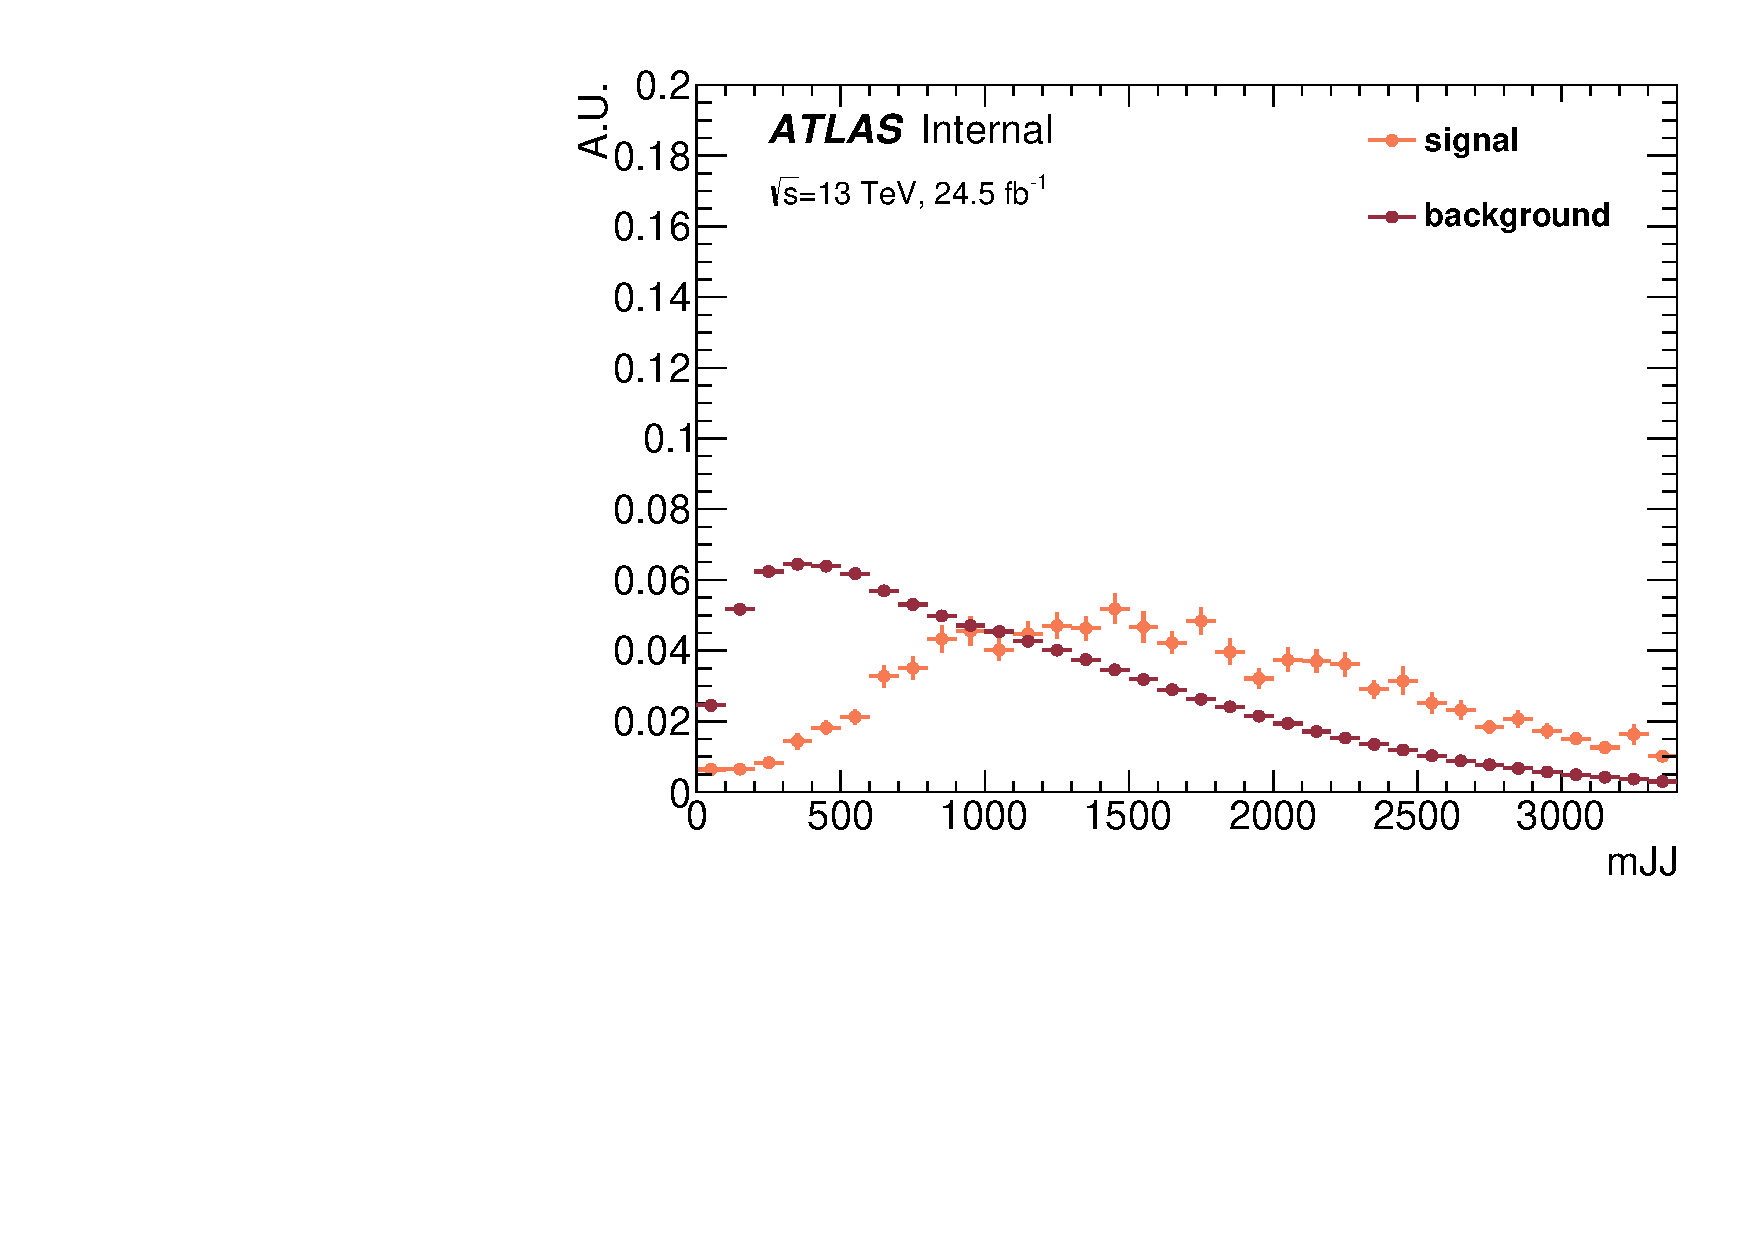
\includegraphics[width=0.3\textwidth]{figures/VBF/BDT_mJJ_2cen.pdf}
 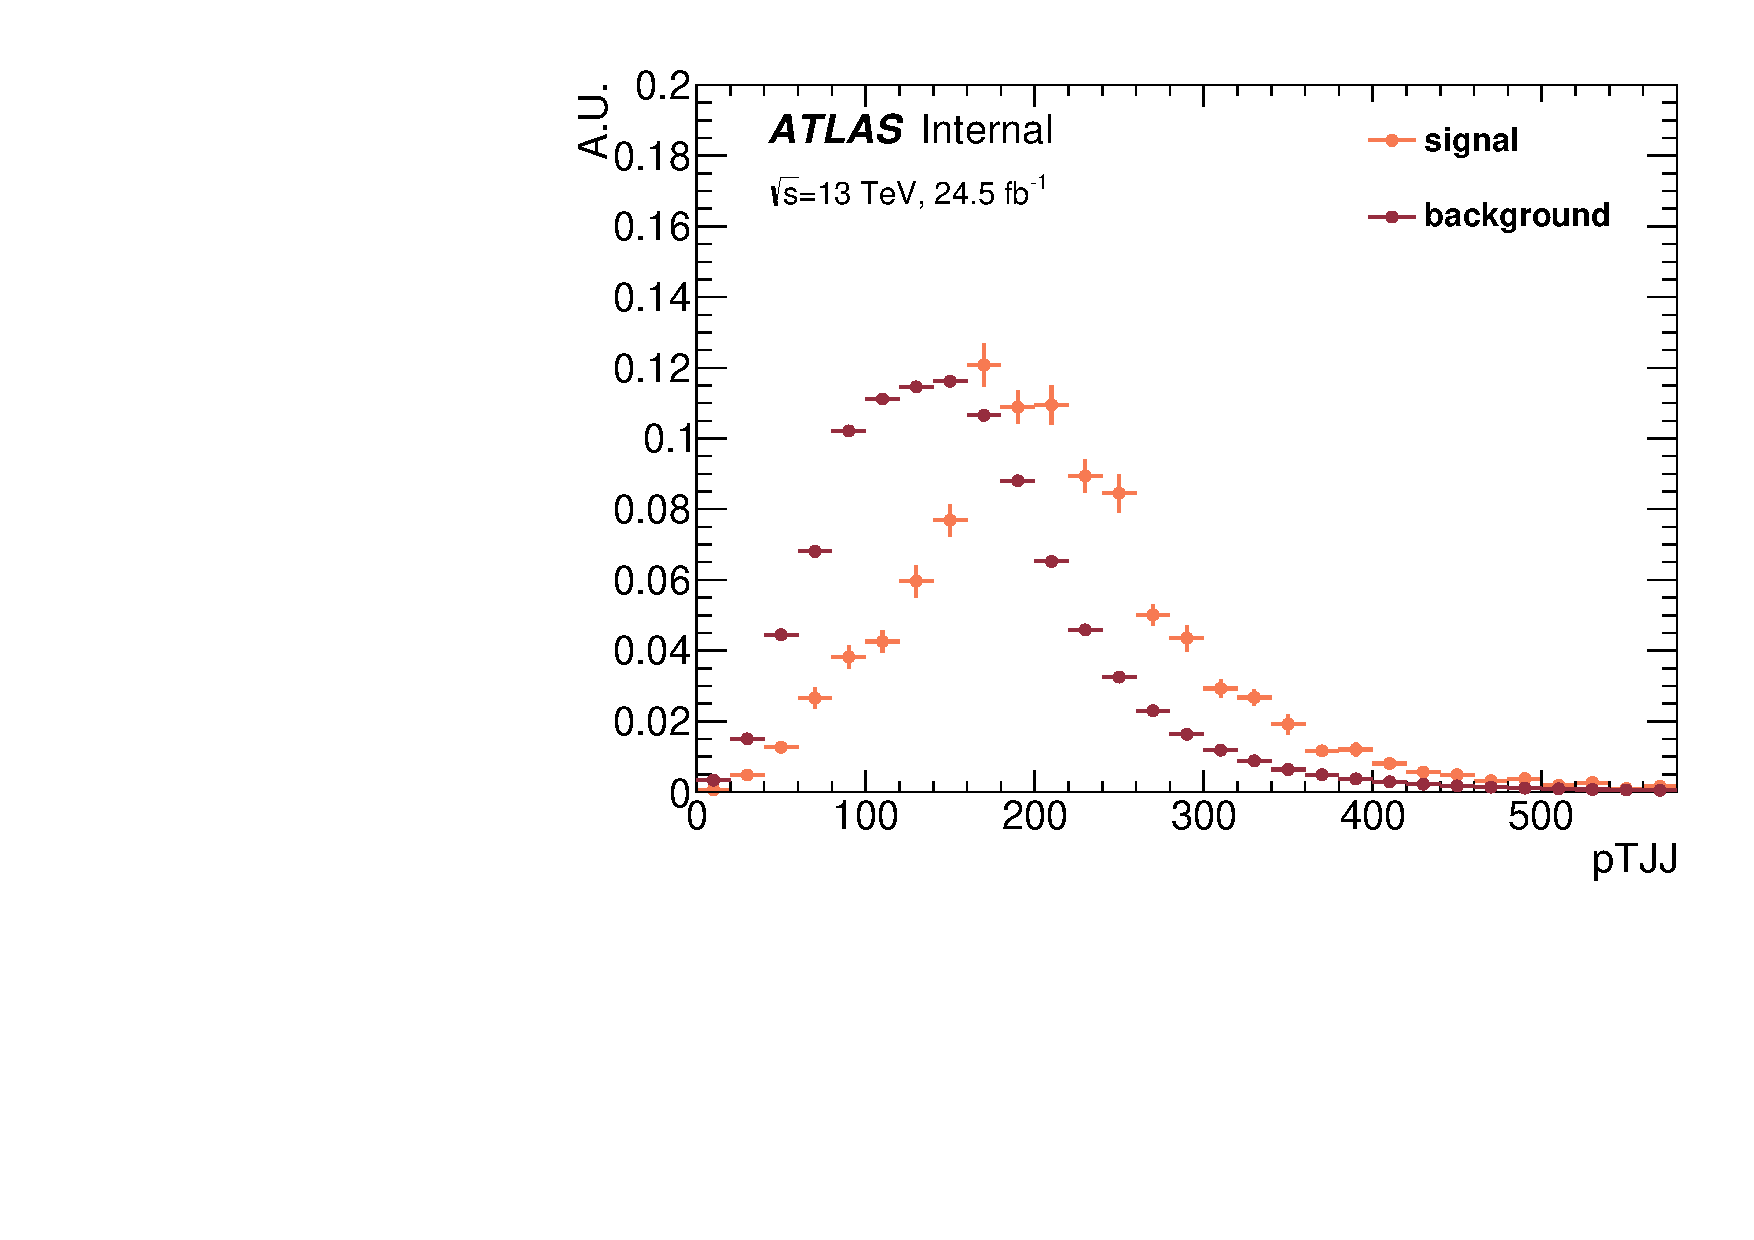
\includegraphics[width=0.3\textwidth]{figures/VBF/BDT_pTJJ_2cen.pdf}
 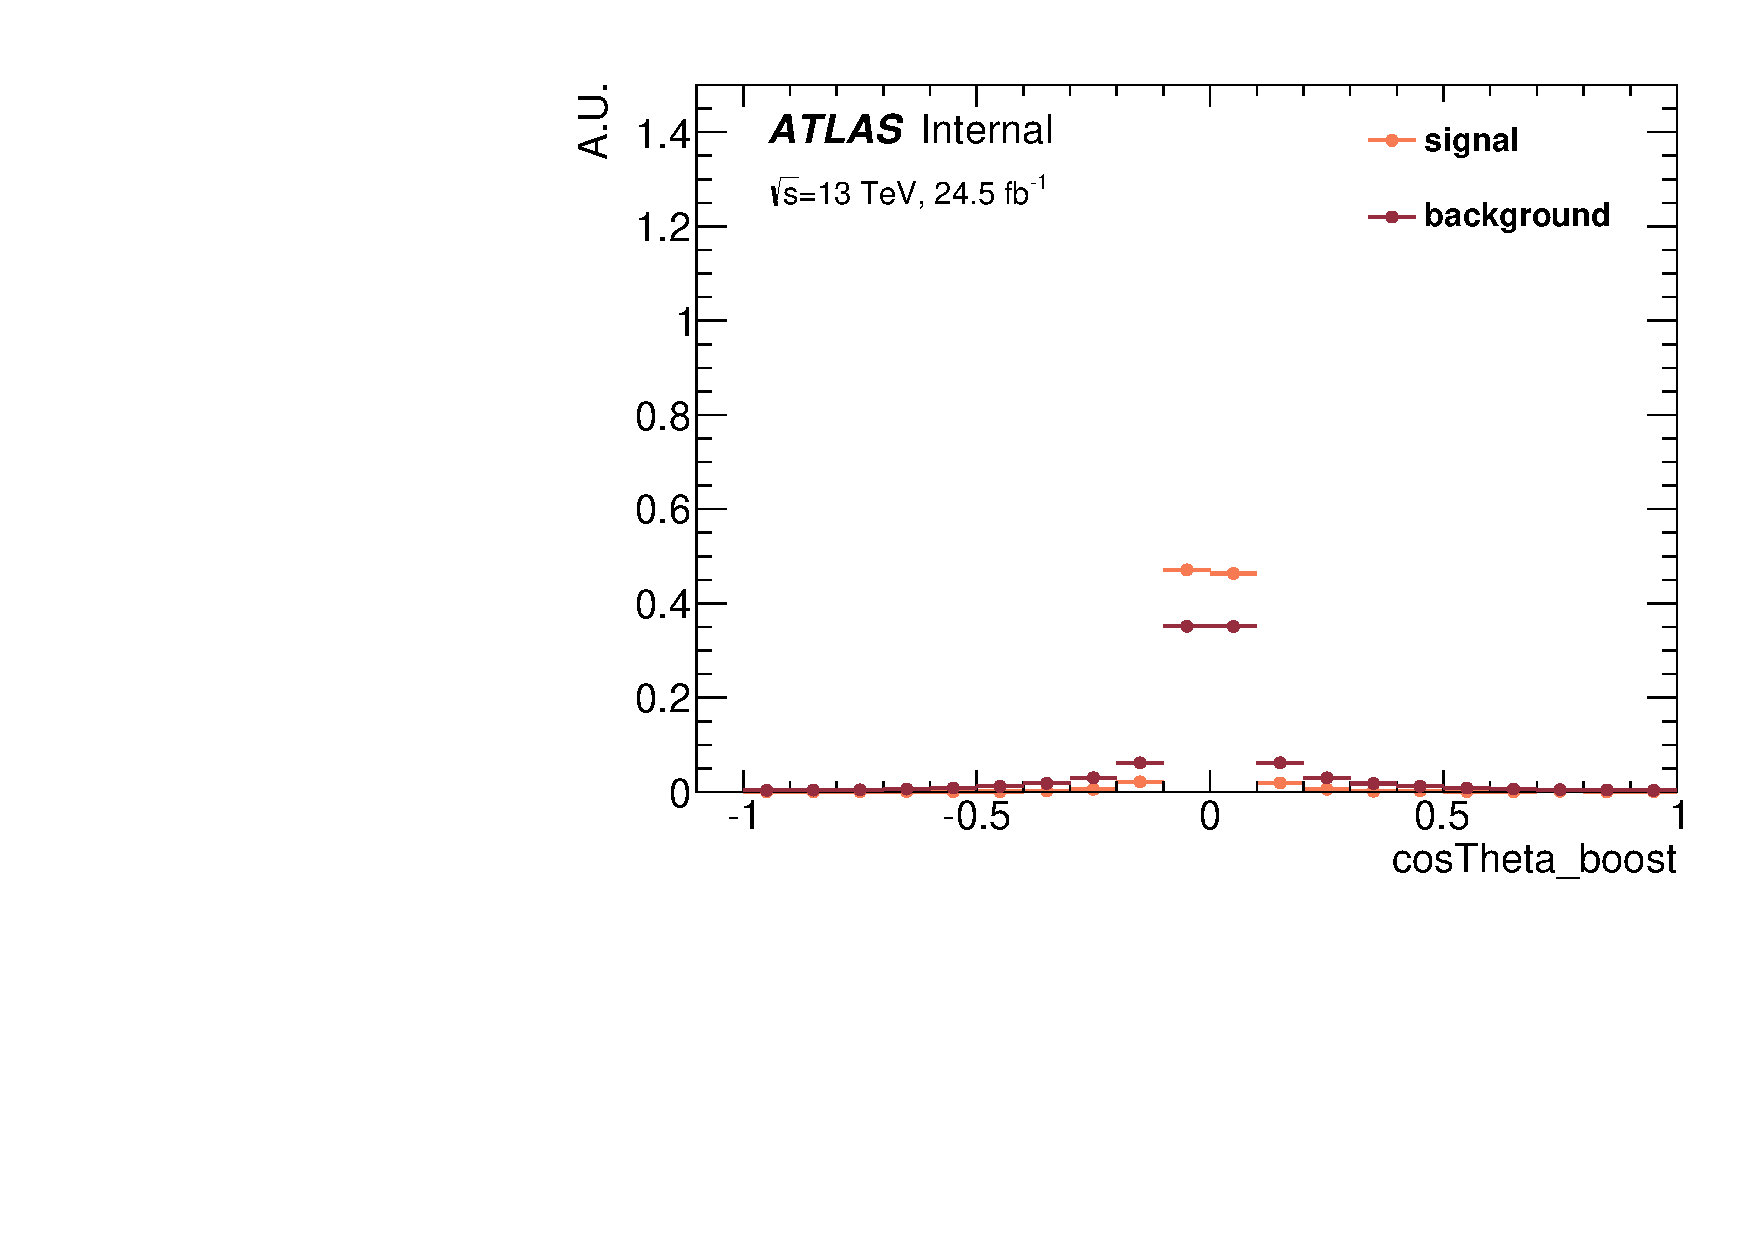
\includegraphics[width=0.3\textwidth]{figures/VBF/BDT_cosTheta_2cen.pdf}\\
 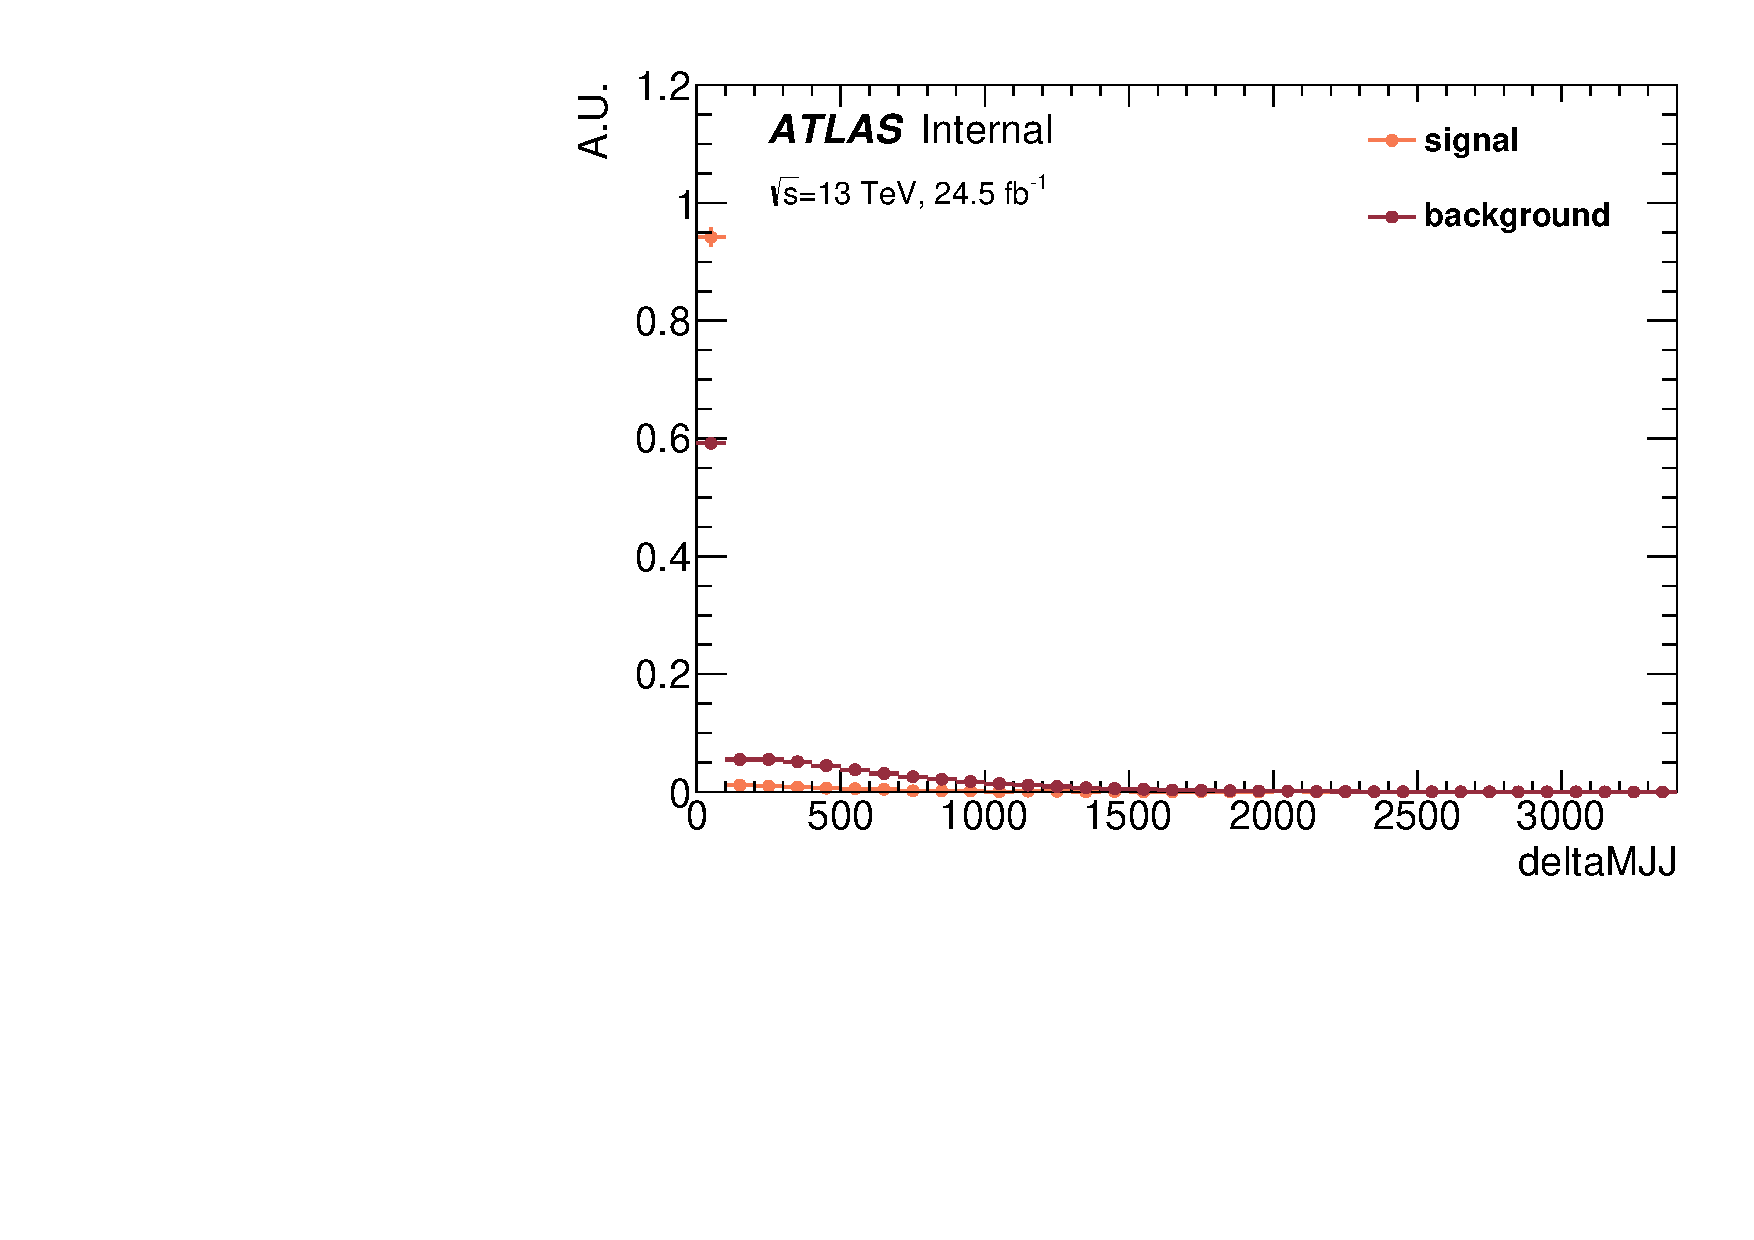
\includegraphics[width=0.3\textwidth]{figures/VBF/BDT_deltaMJJ_2cen.pdf}
 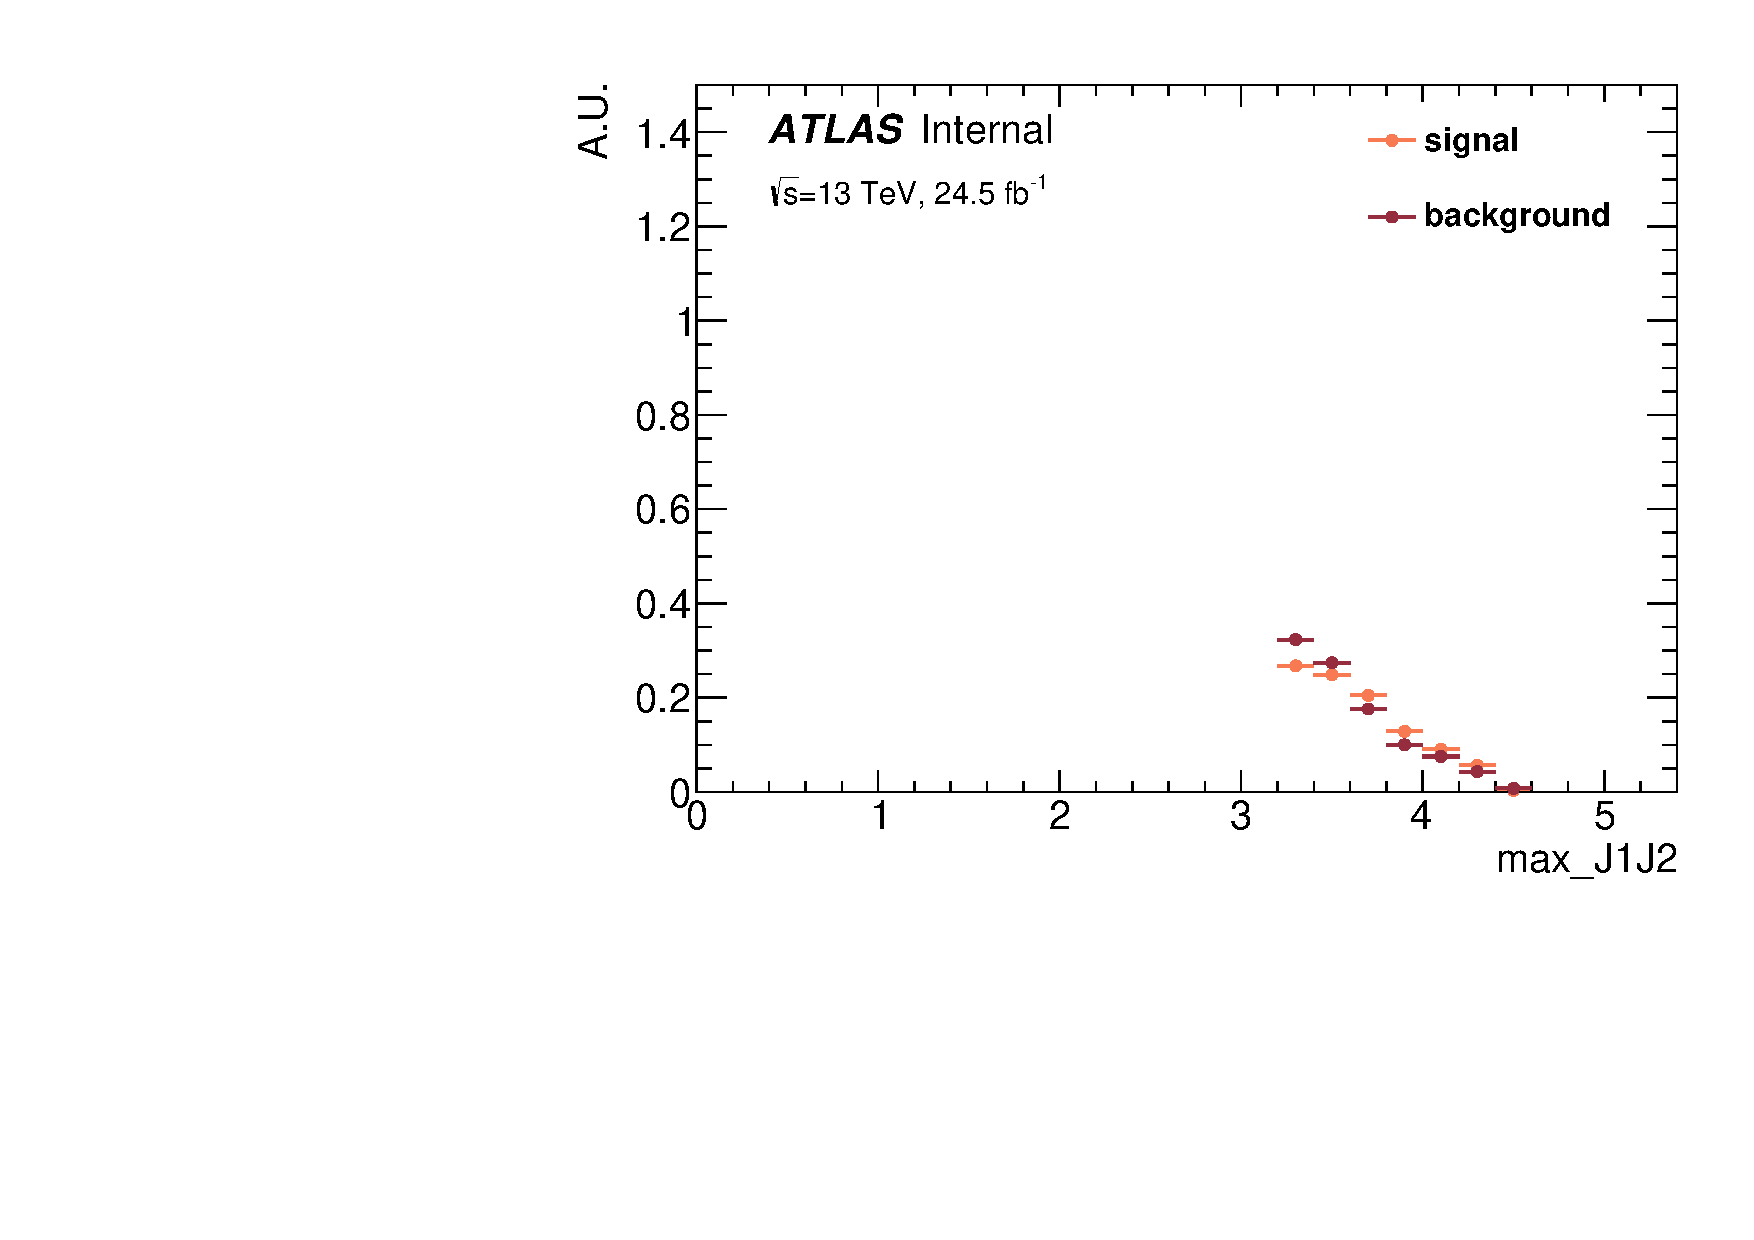
\includegraphics[width=0.3\textwidth]{figures/VBF/BDT_maxJ1J2_2cen.pdf}
 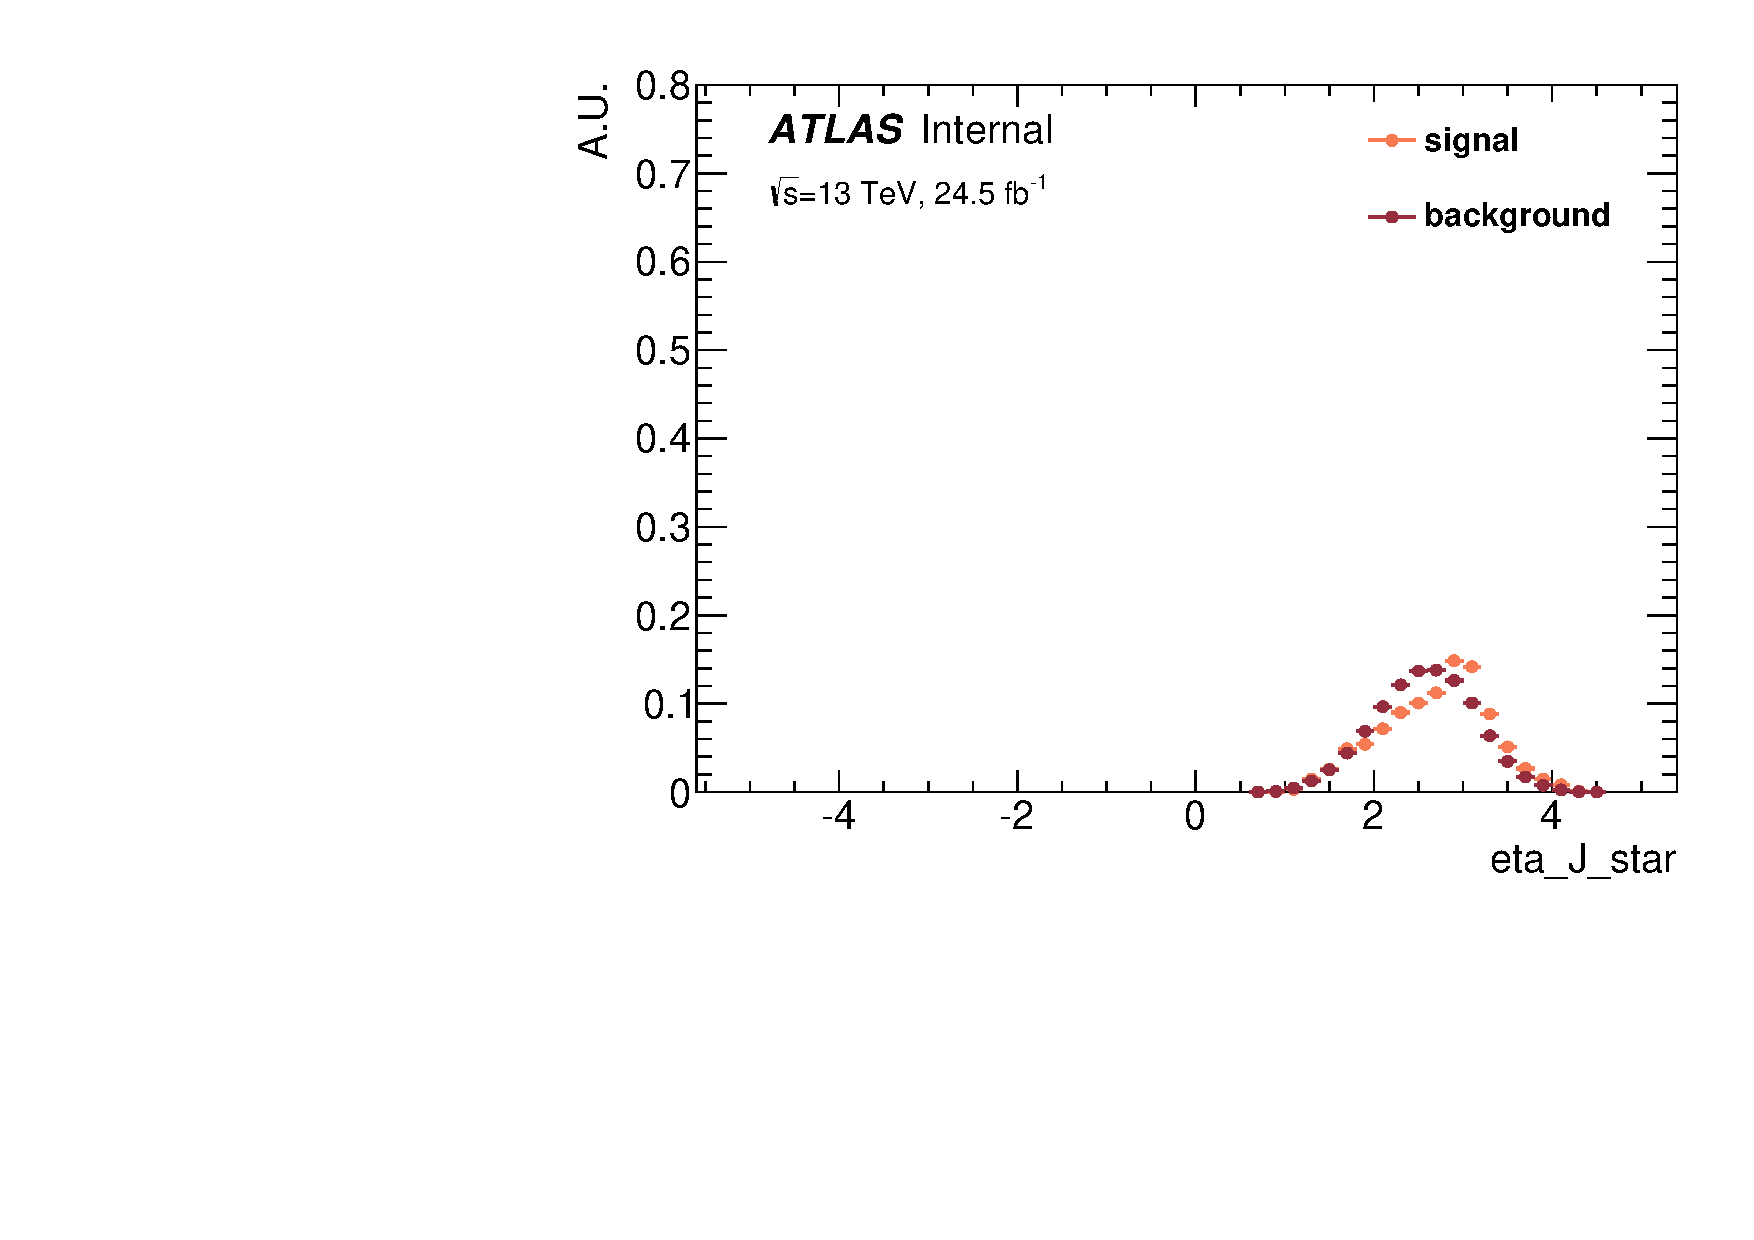
\includegraphics[width=0.3\textwidth]{figures/VBF/BDT_etaJstar_2cen.pdf}\\
 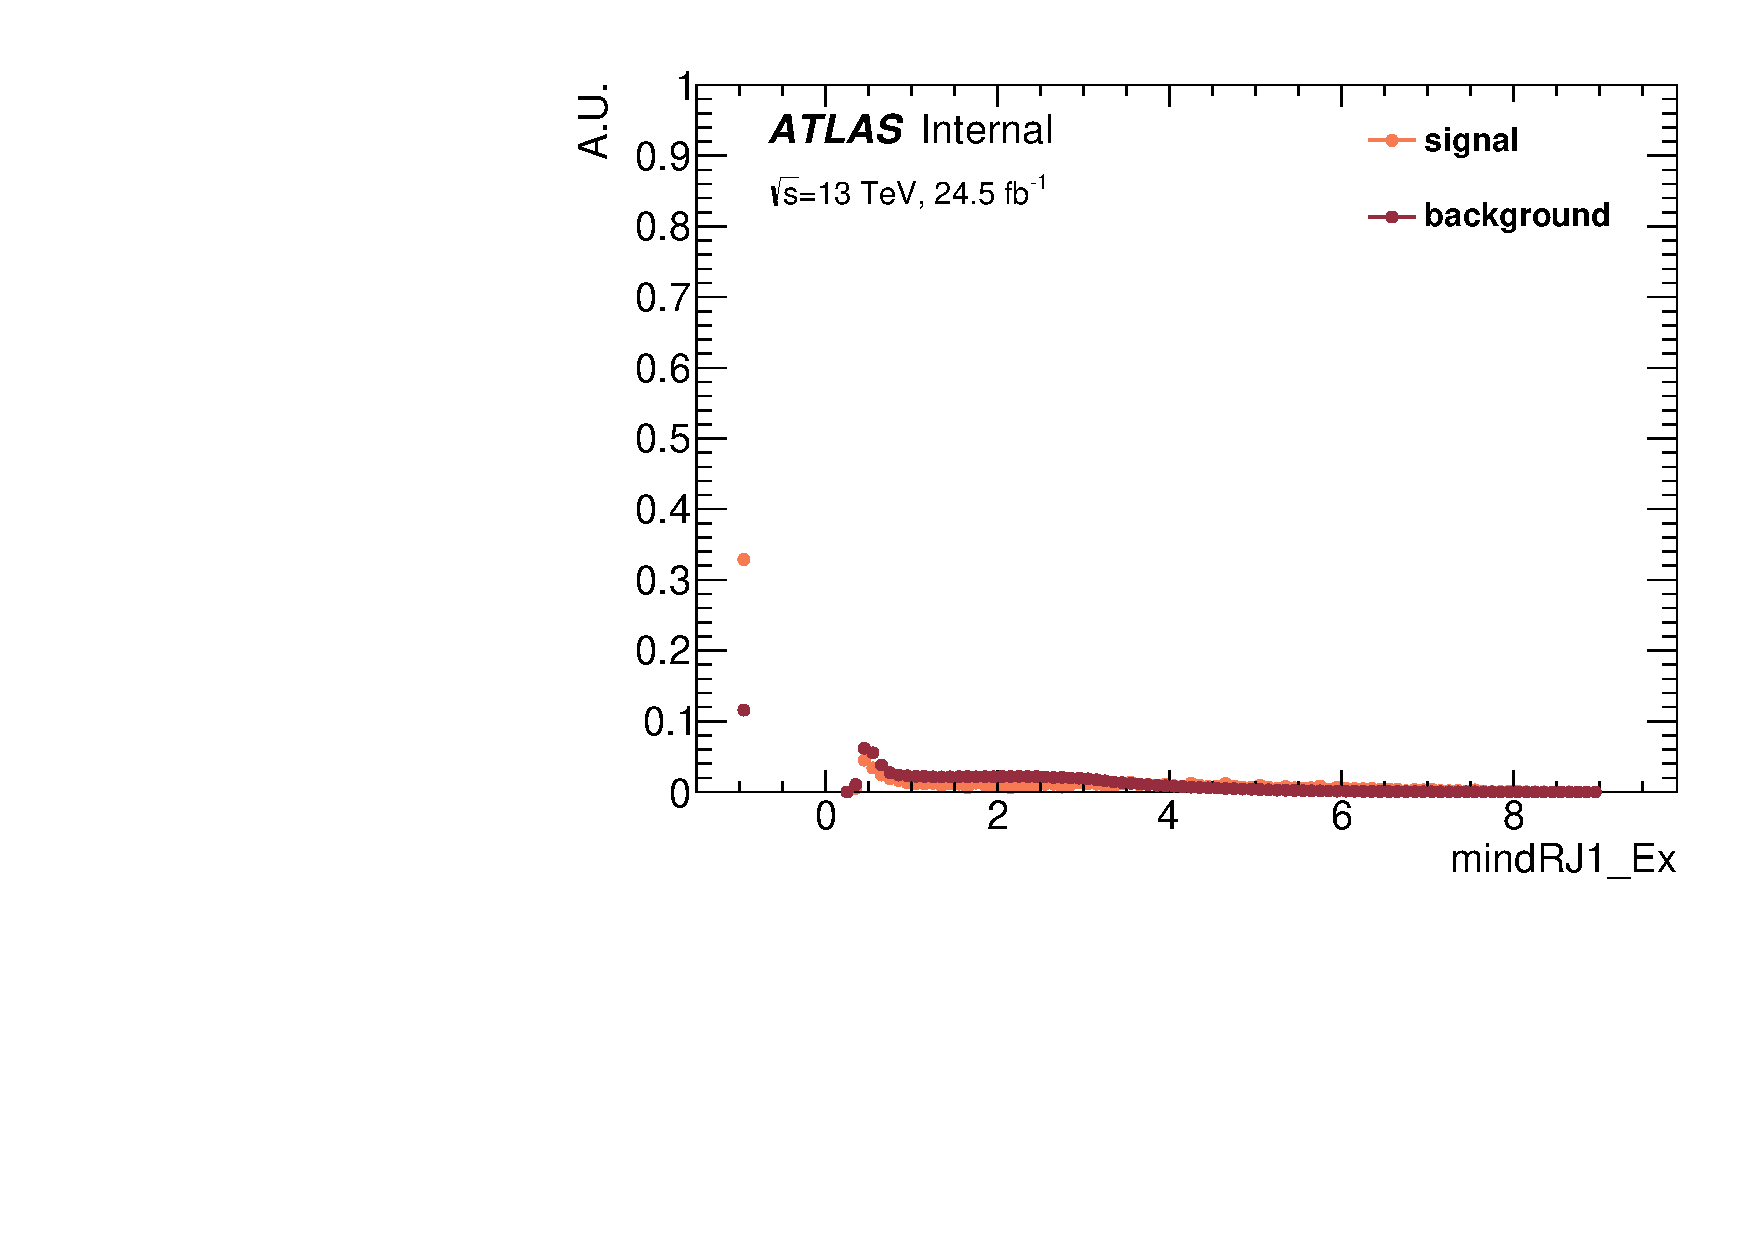
\includegraphics[width=0.3\textwidth]{figures/VBF/BDT_mindRJ1_2cen.pdf}
 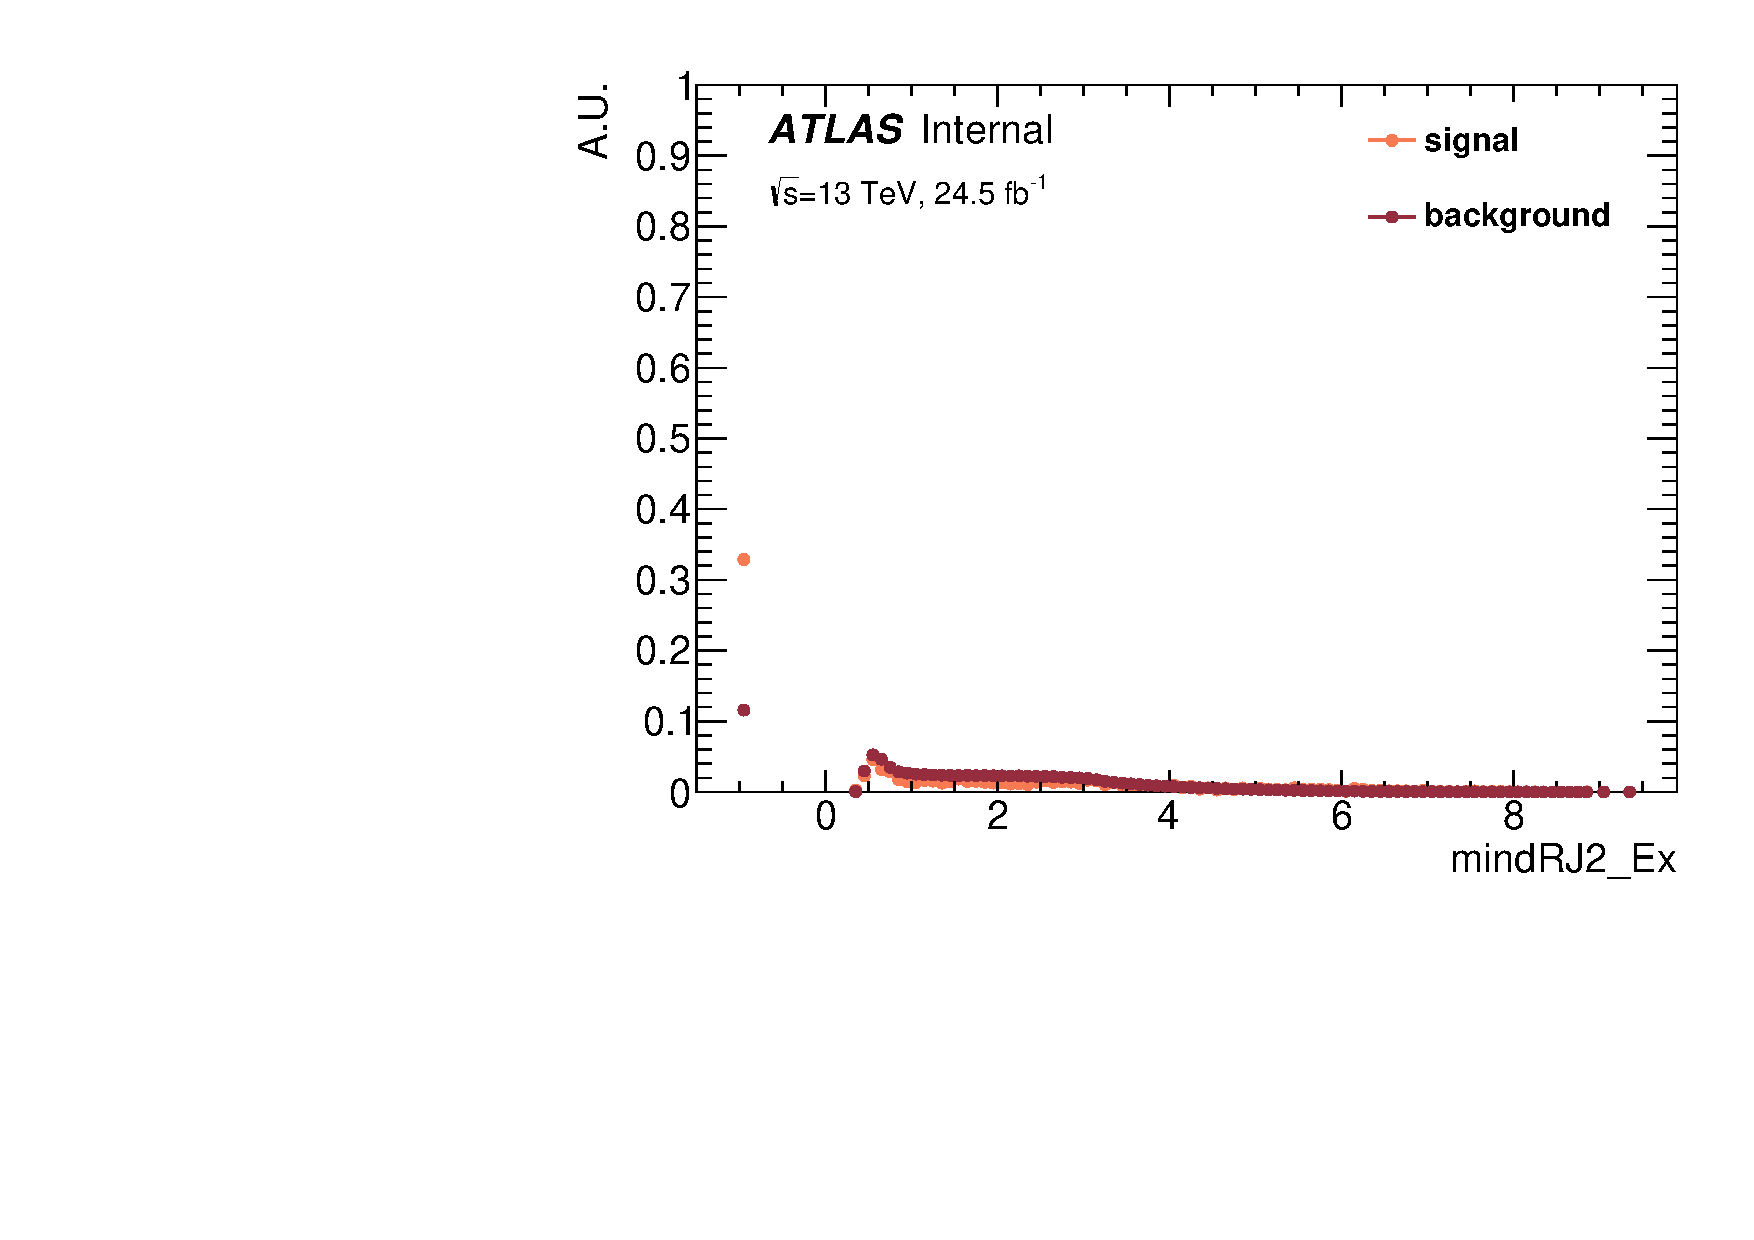
\includegraphics[width=0.3\textwidth]{figures/VBF/BDT_mindRJ2_2cen.pdf}
 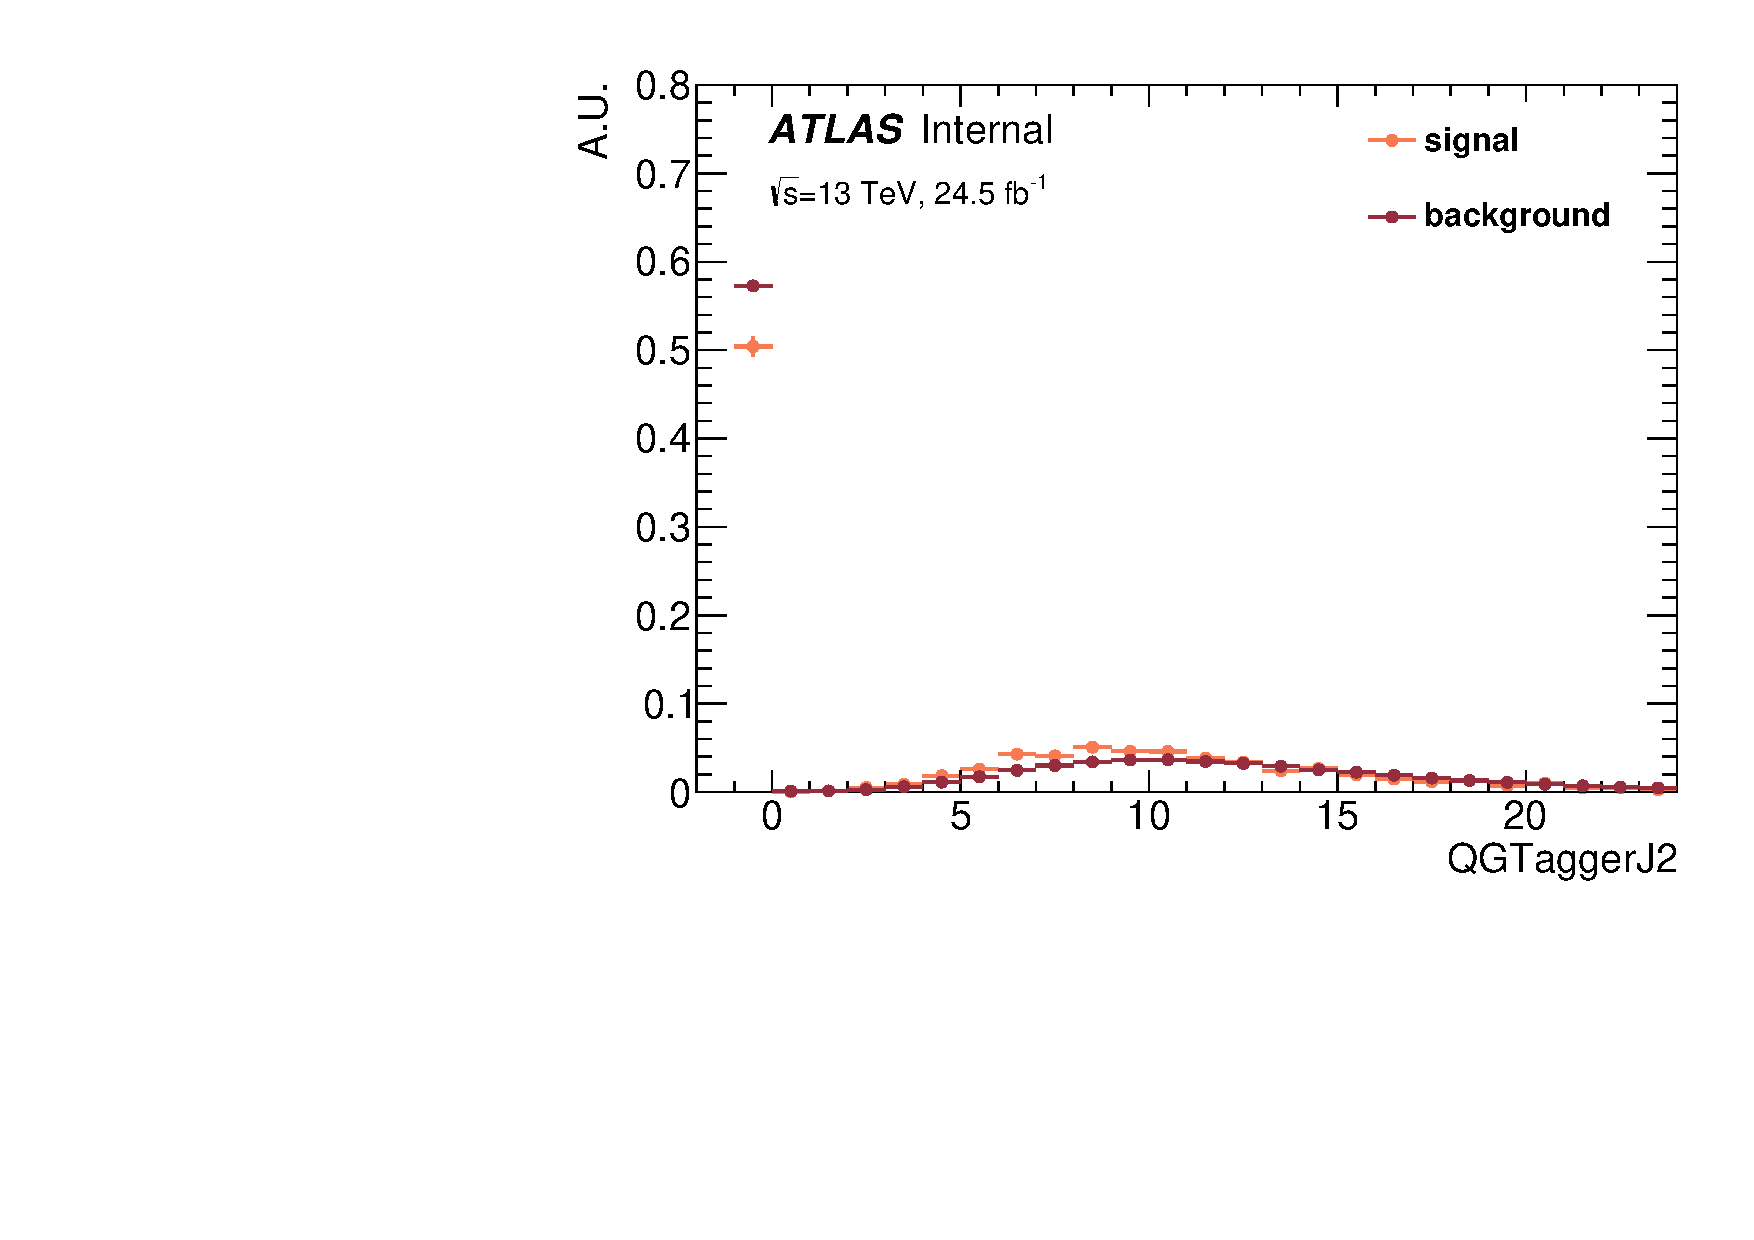
\includegraphics[width=0.3\textwidth]{figures/VBF/BDT_NTrk500_J2_2cen.pdf}\\
 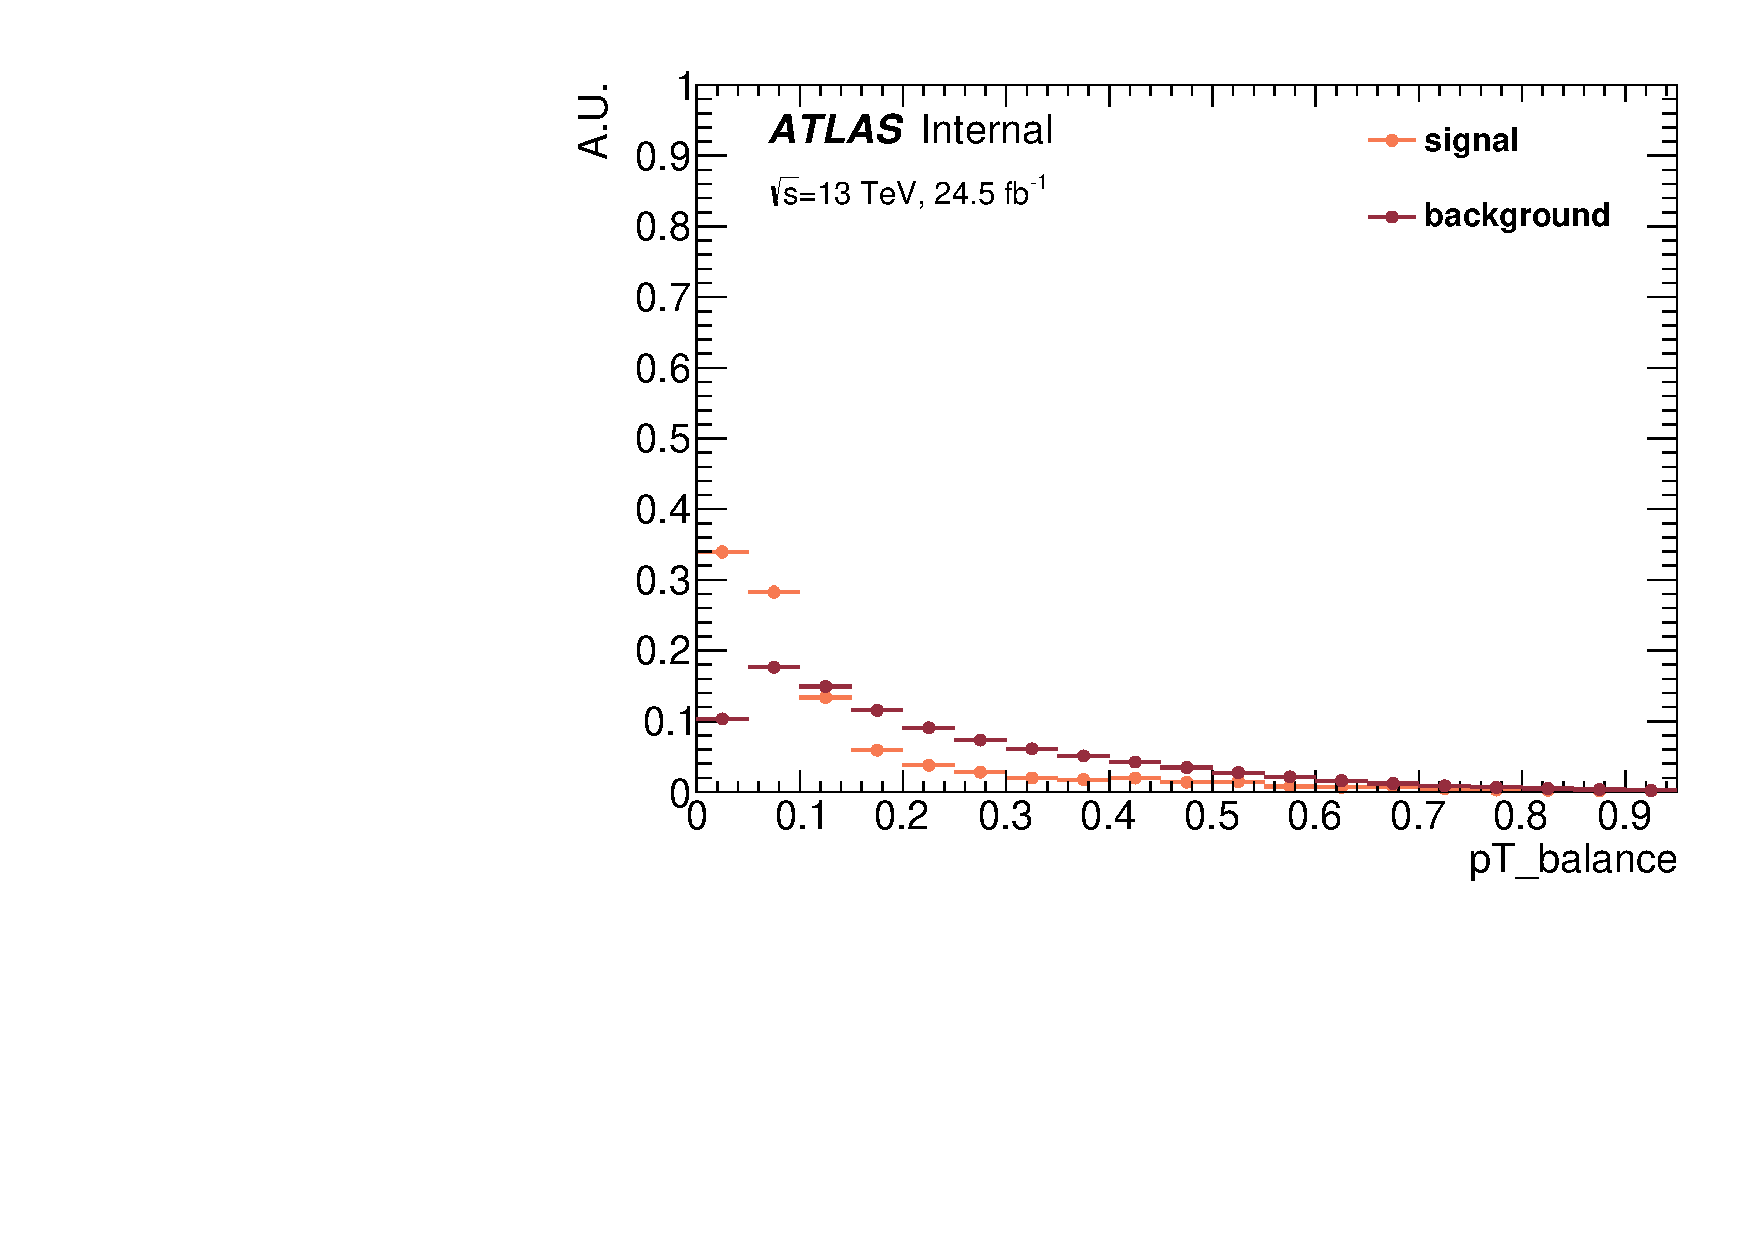
\includegraphics[width=0.3\textwidth]{figures/VBF/BDT_pTBalance_2cen.pdf}\\

 %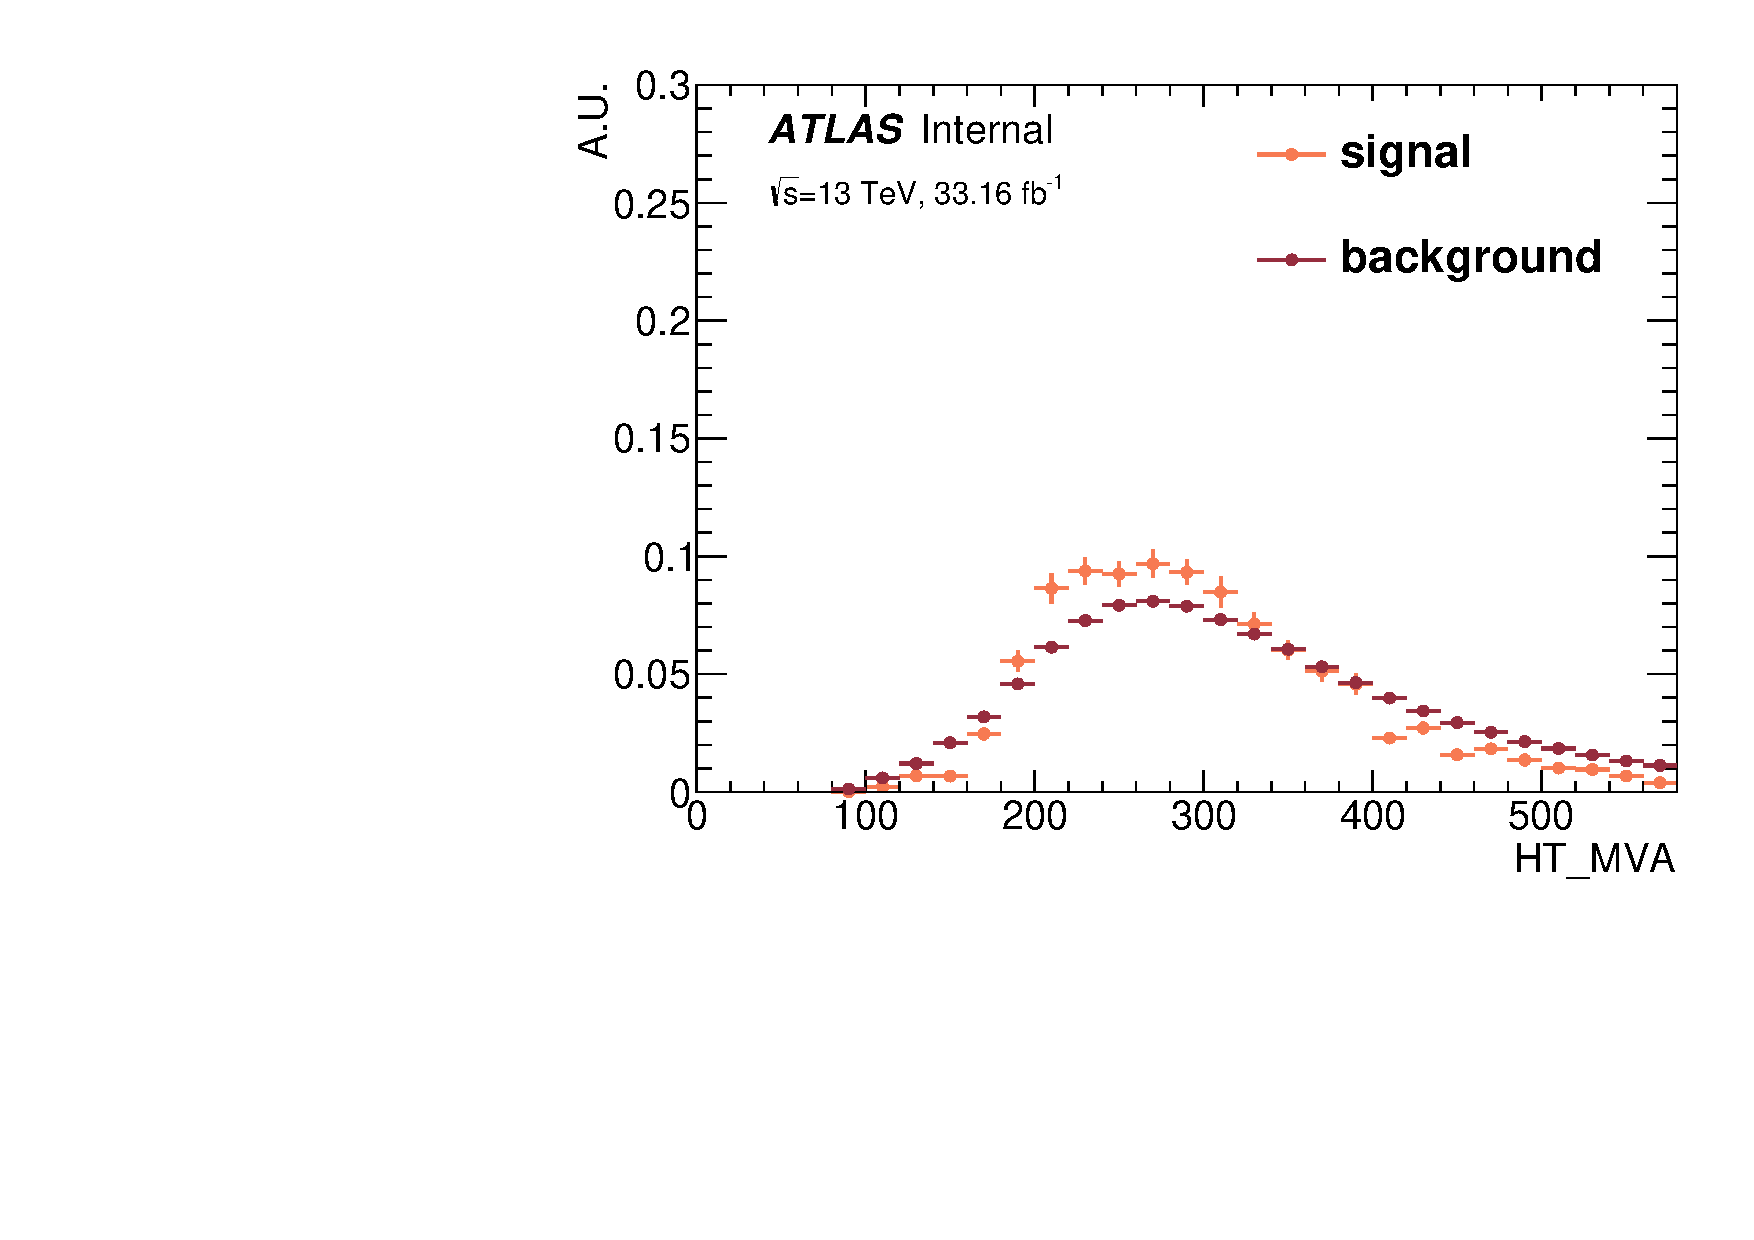
\includegraphics[width=0.3\textwidth]{figures/VBF/BDT_HT_2cen.pdf}
\caption{Distributions of BDT input variables of \twocentral channel.  $N_{\rm Trk}($J1$)PV500$ is identically zero because J1 is by definition outside of the tracker acceptance.}
  \label{fig:vbf-BDTInputs2cen}
\end{figure}

\begin{figure}[htbp]
  \centering
 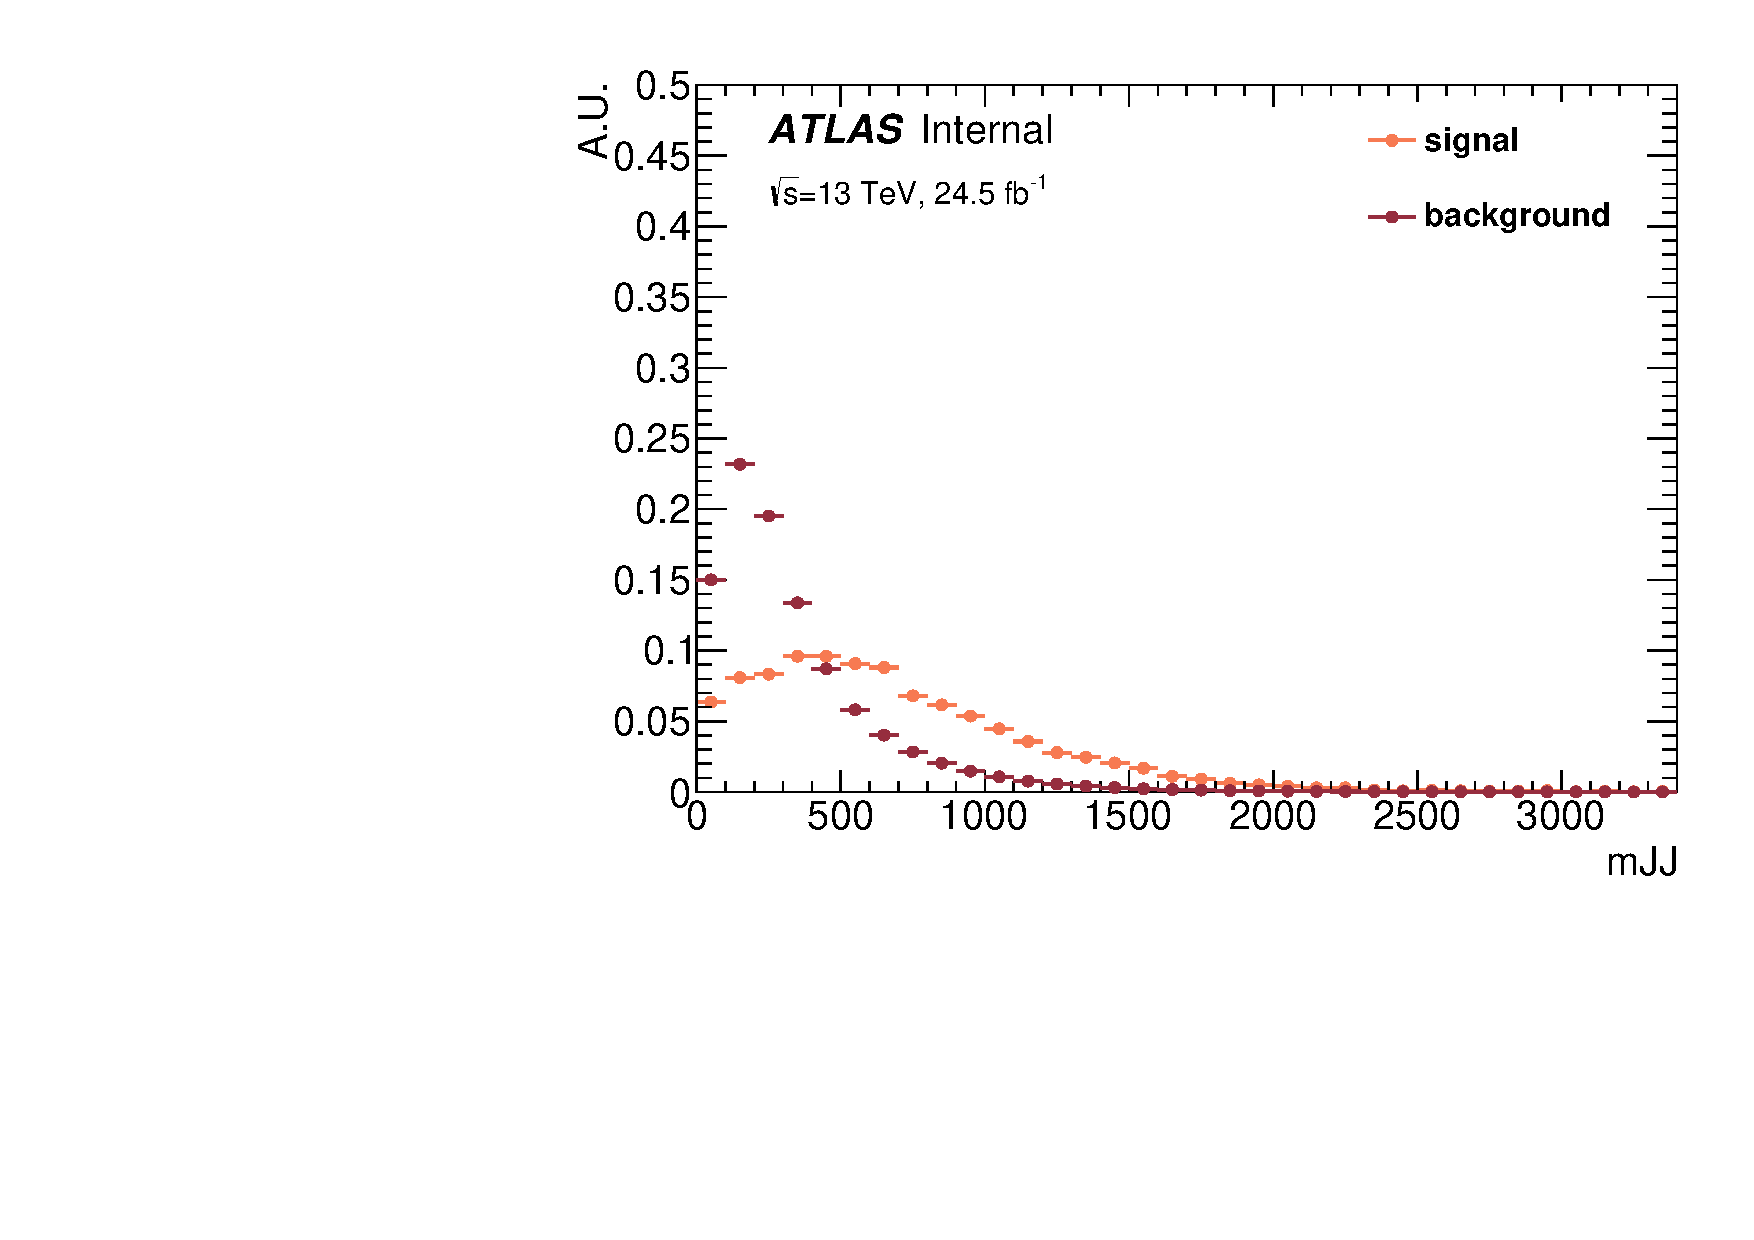
\includegraphics[width=0.3\textwidth]{figures/VBF/BDT_mJJ_4cen.pdf}
 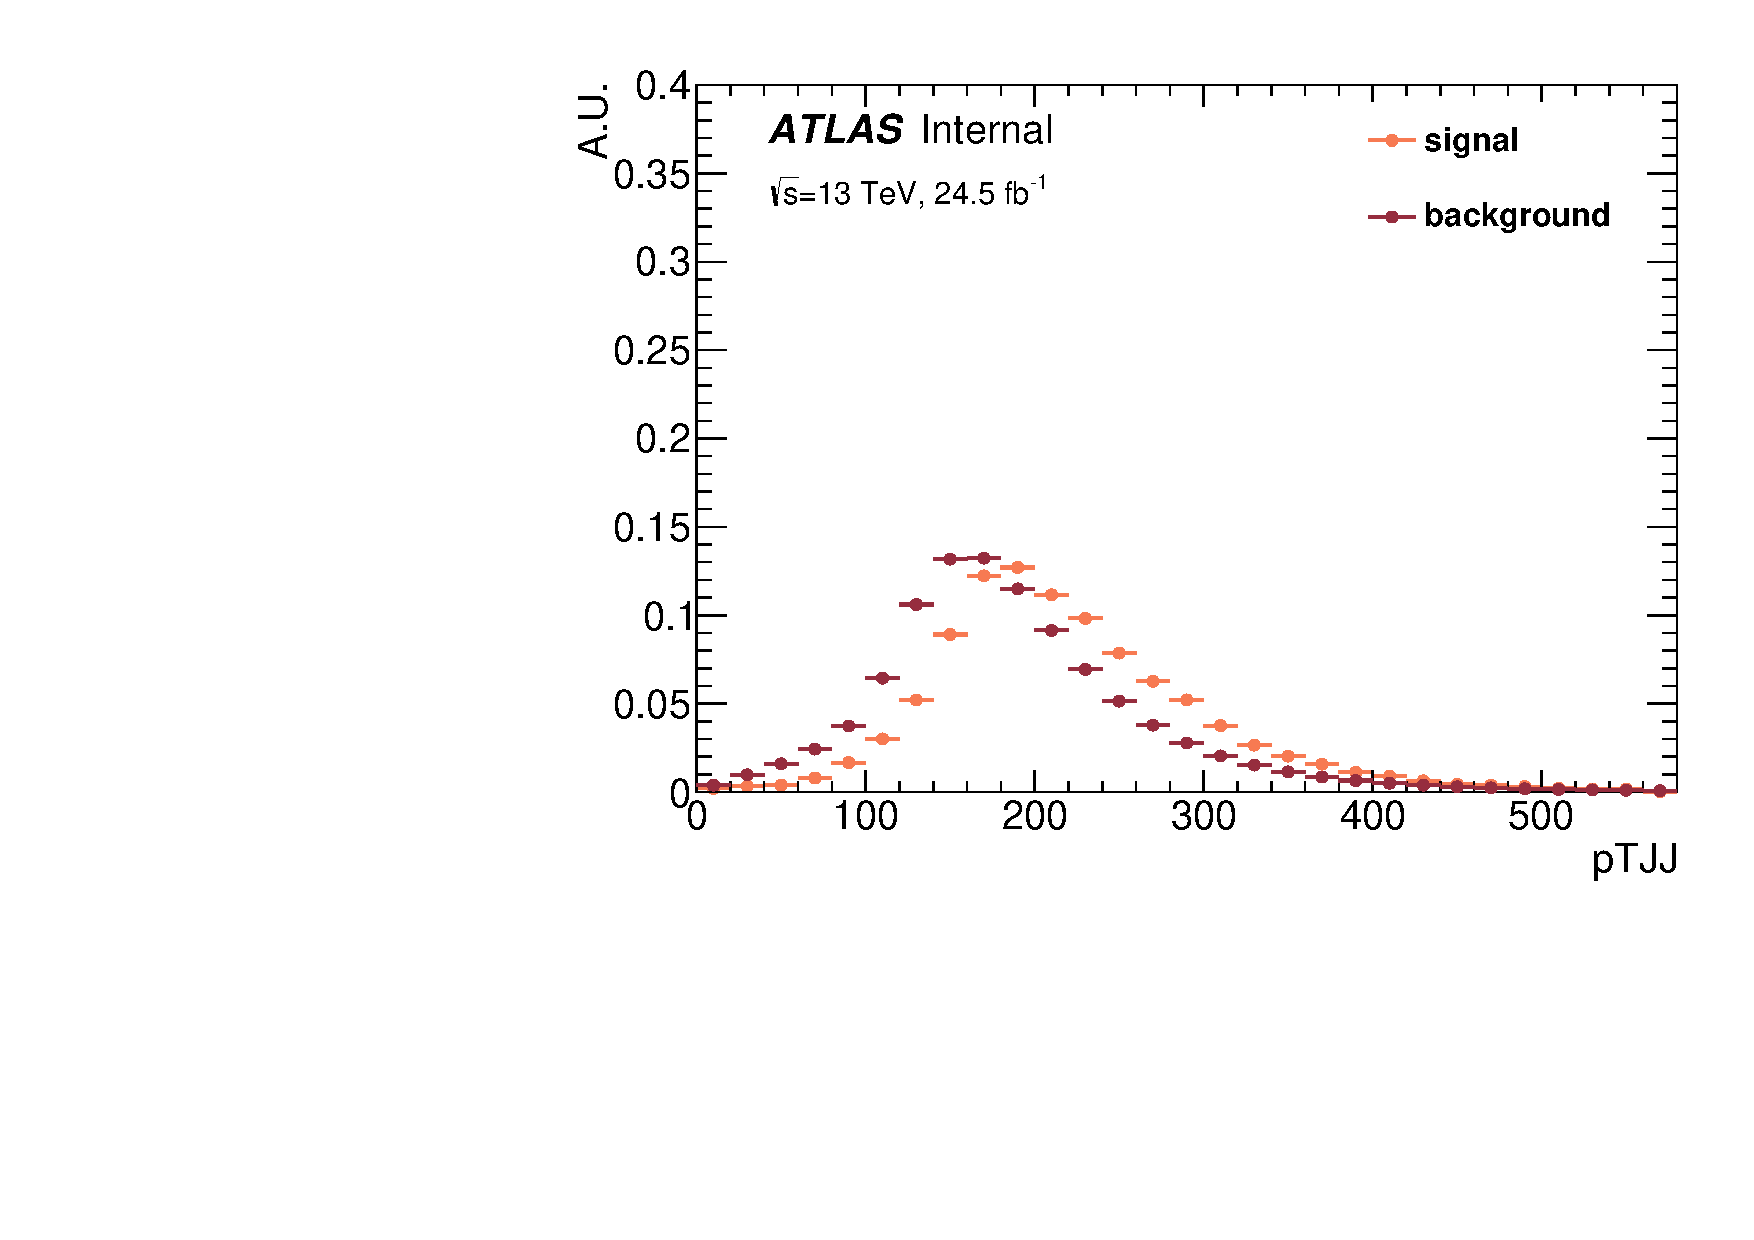
\includegraphics[width=0.3\textwidth]{figures/VBF/BDT_pTJJ_4cen.pdf}
 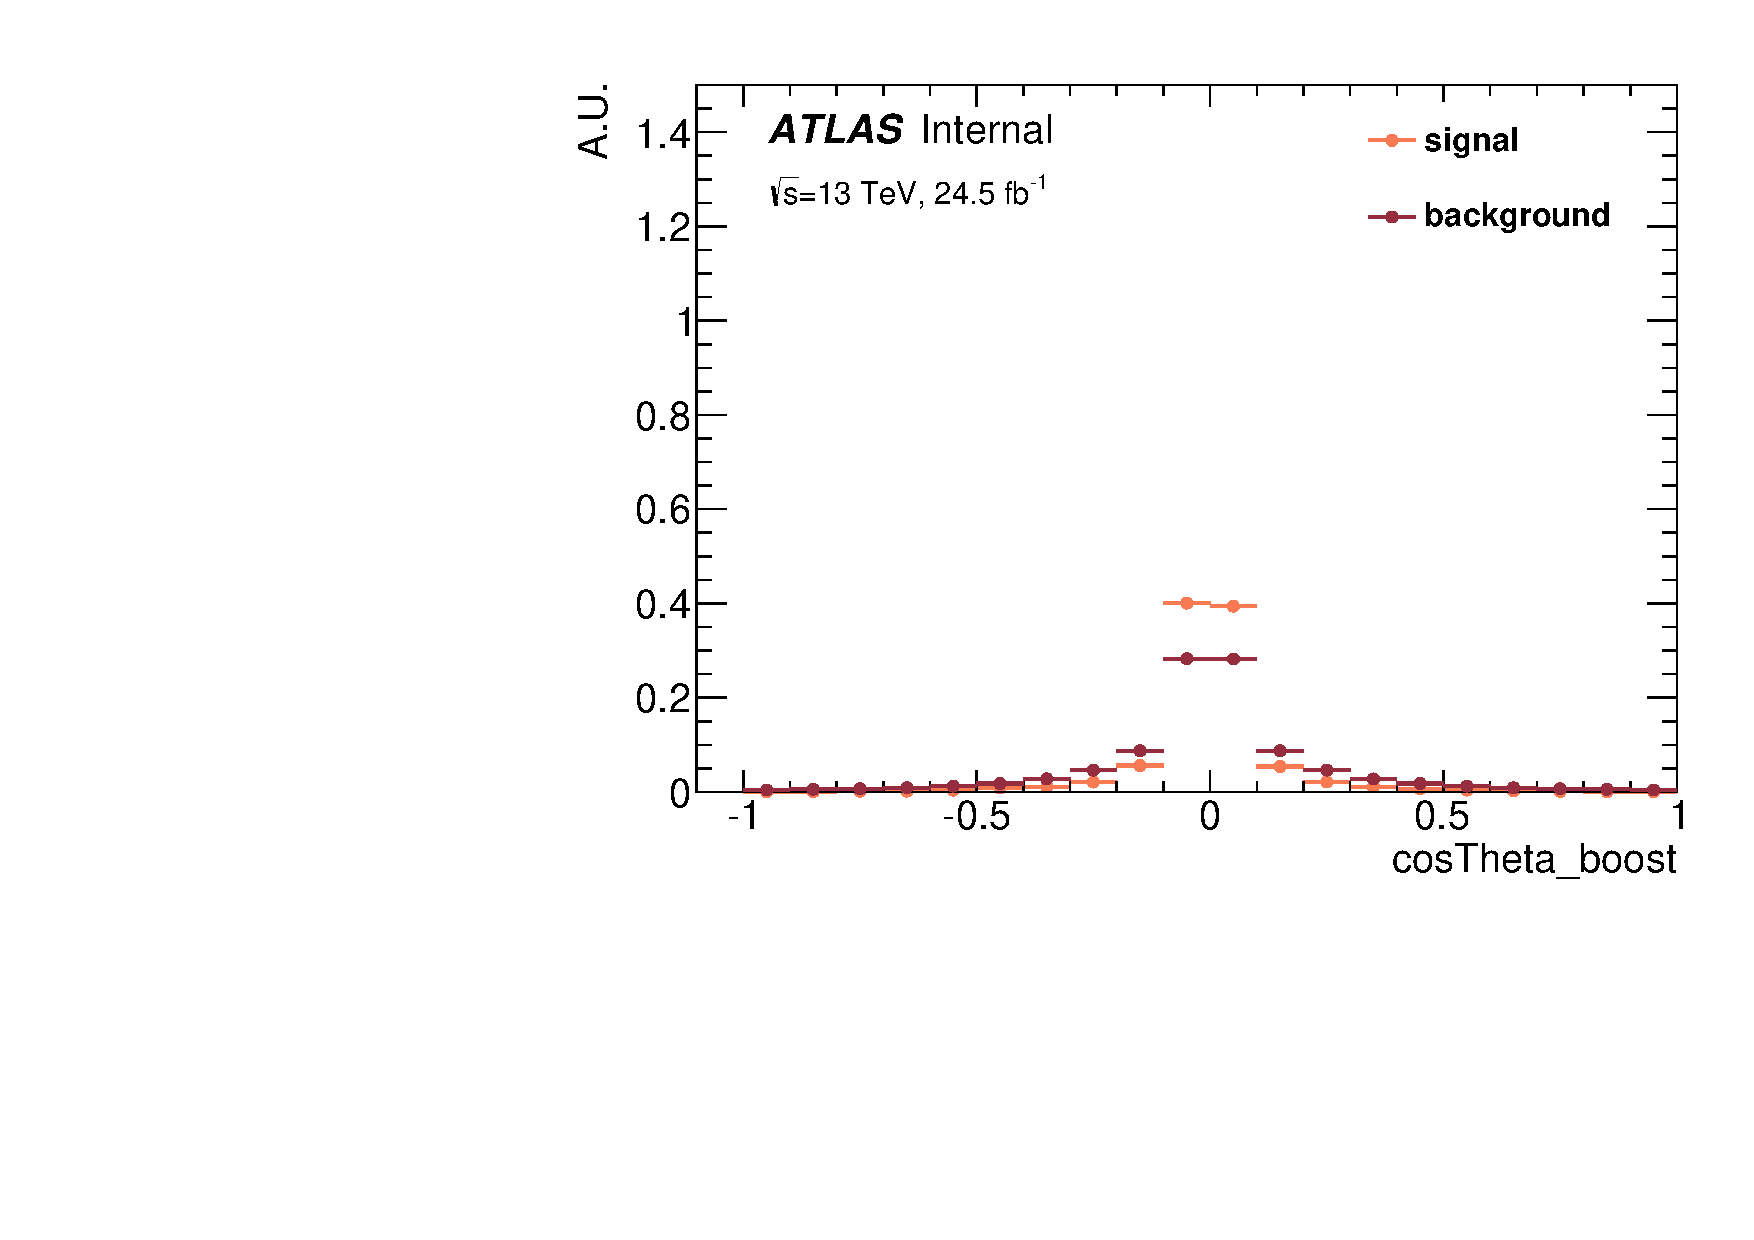
\includegraphics[width=0.3\textwidth]{figures/VBF/BDT_cosTheta_4cen.pdf}\\
 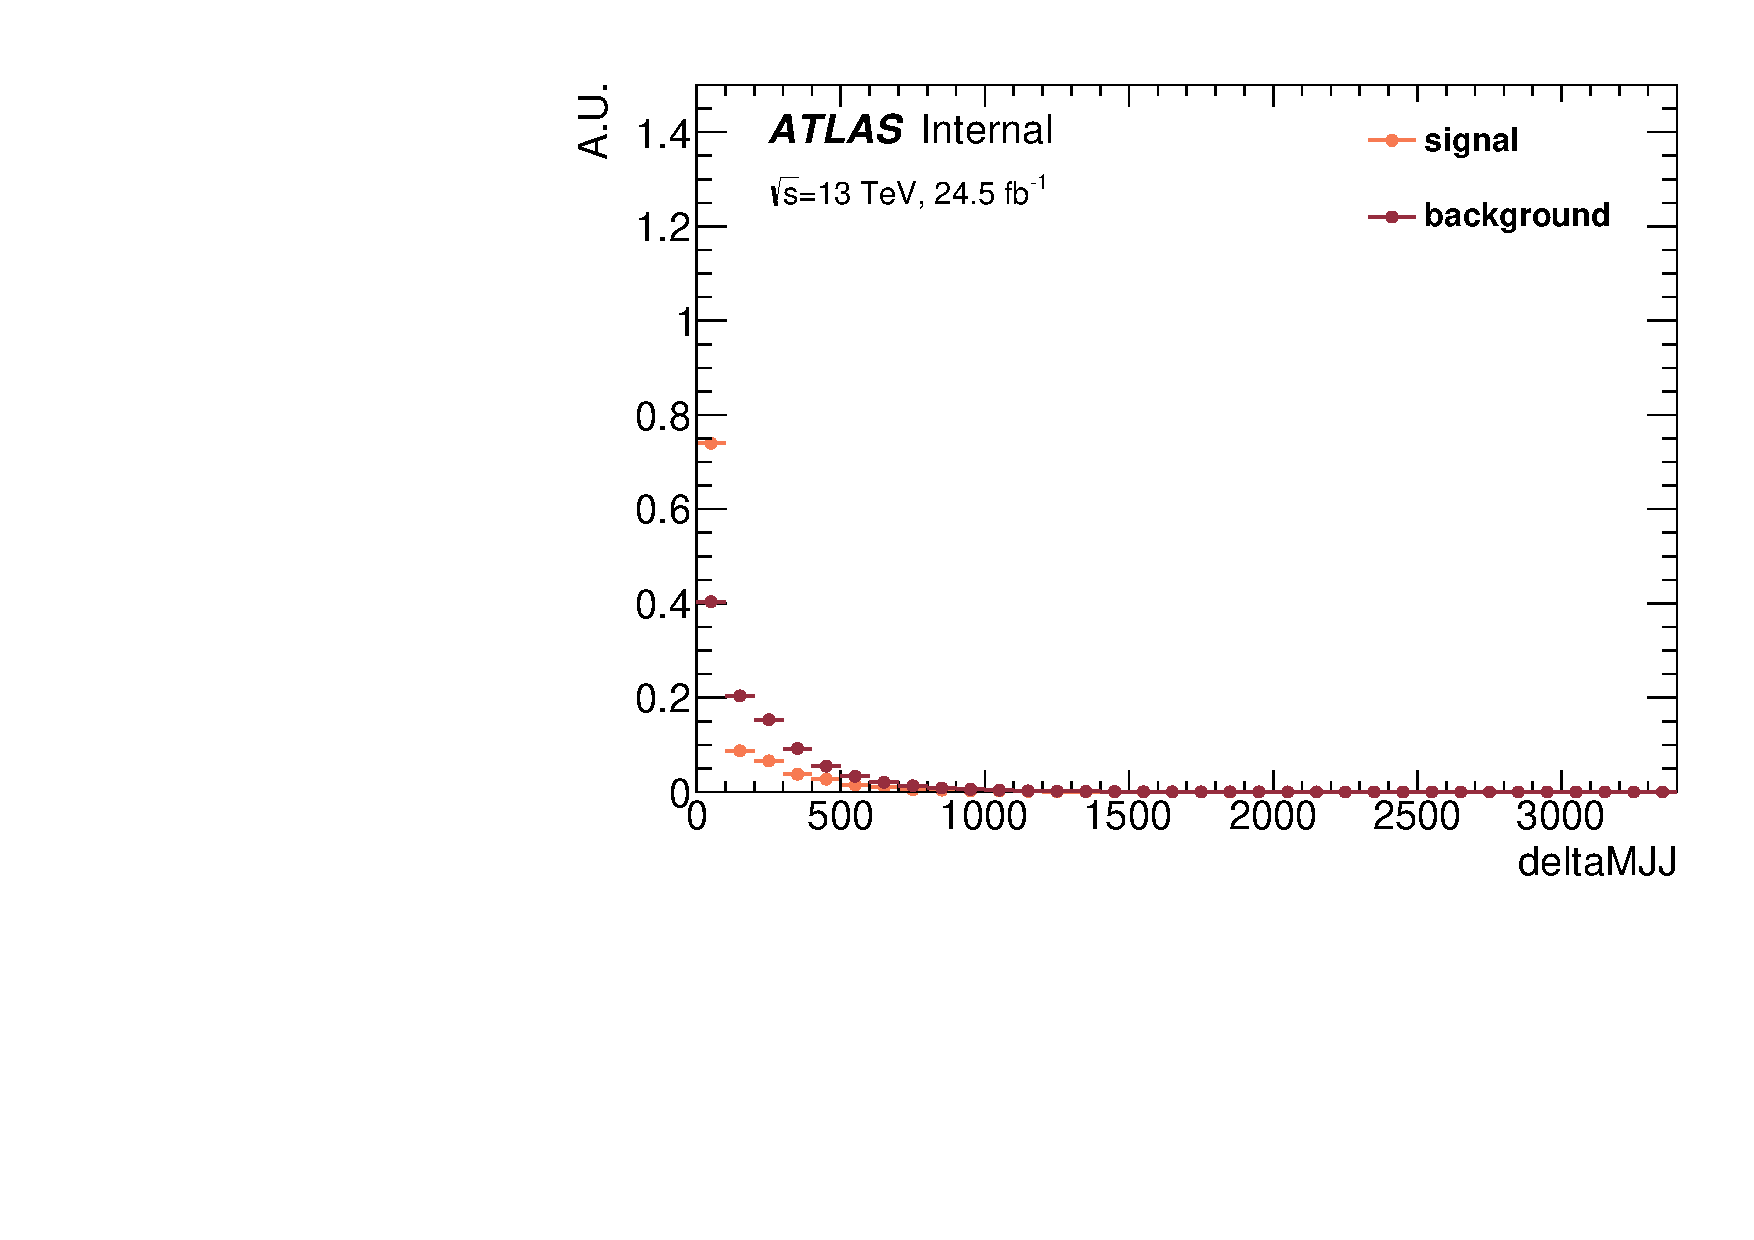
\includegraphics[width=0.3\textwidth]{figures/VBF/BDT_deltaMJJ_4cen.pdf}
 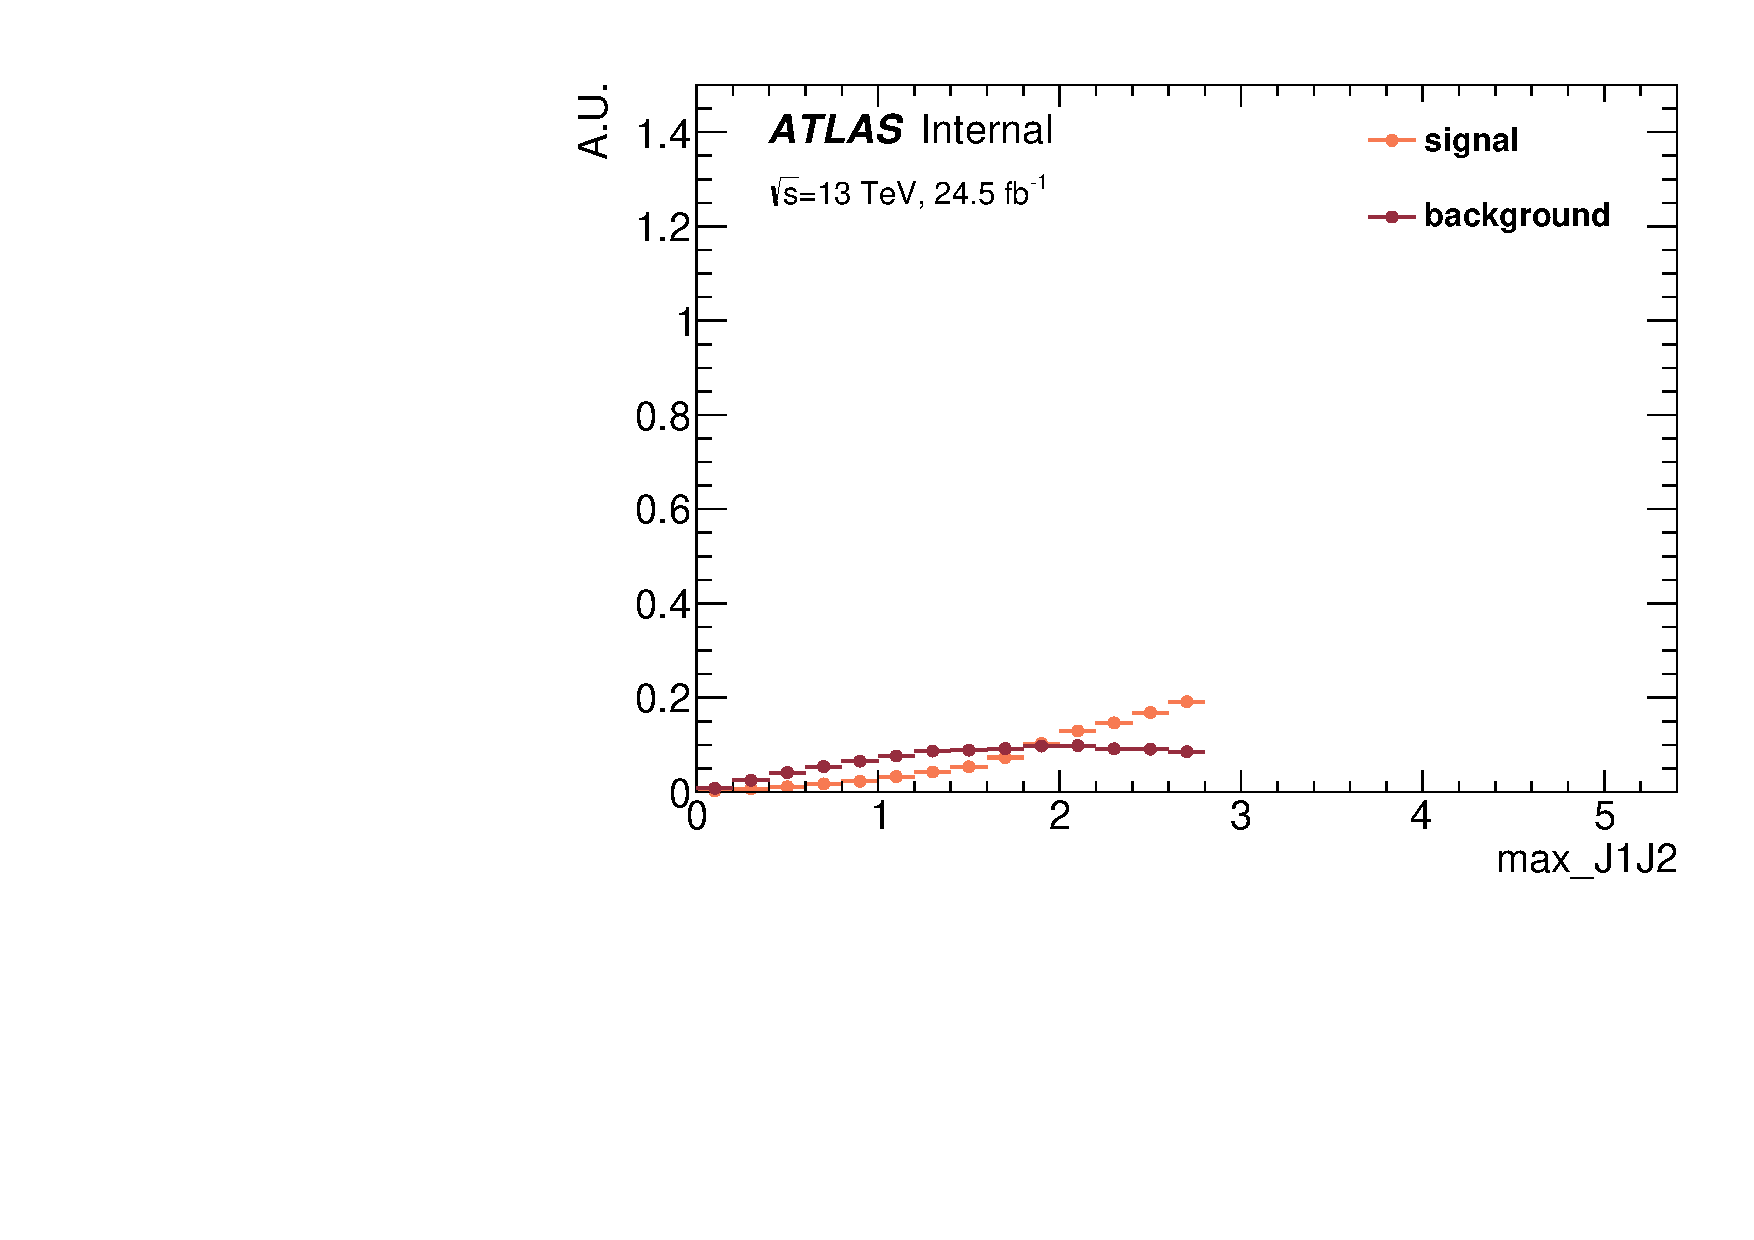
\includegraphics[width=0.3\textwidth]{figures/VBF/BDT_maxJ1J2_4cen.pdf}
 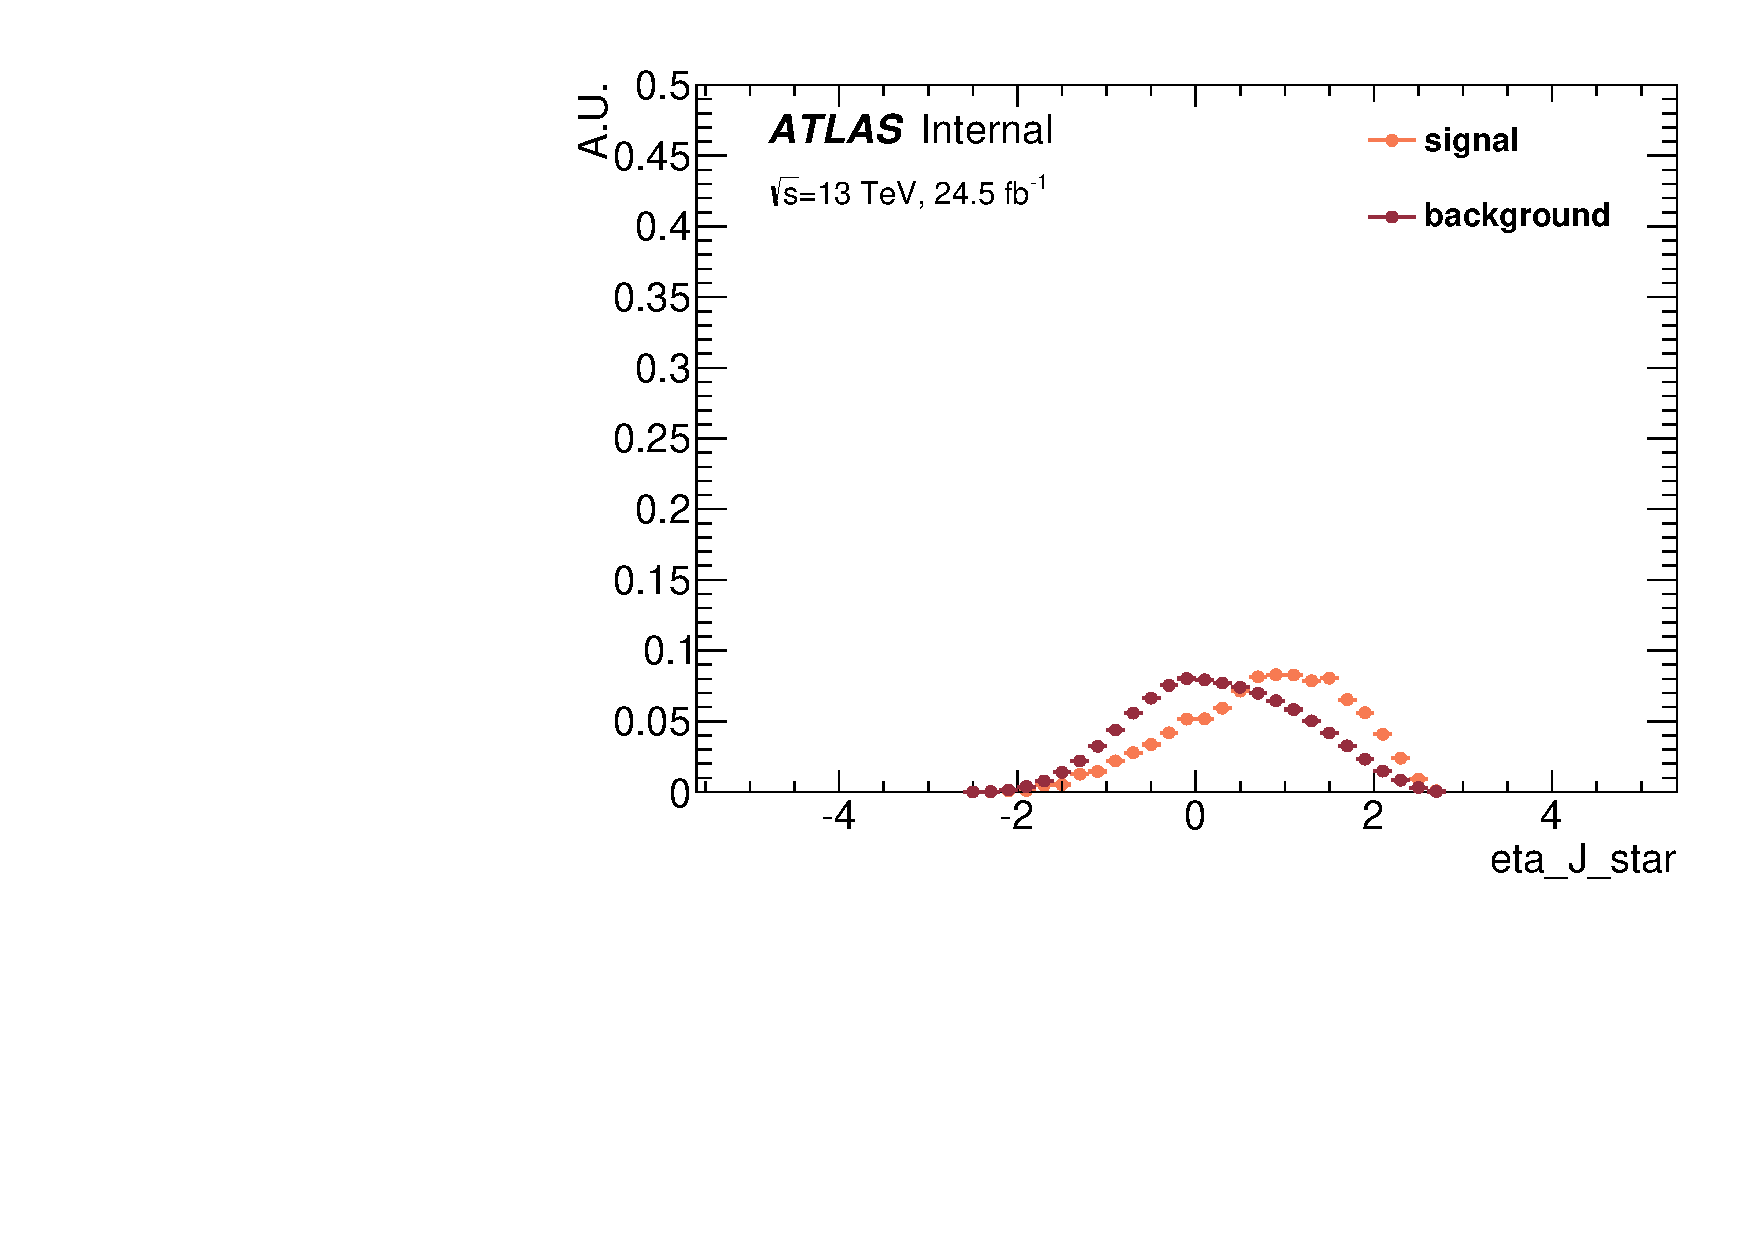
\includegraphics[width=0.3\textwidth]{figures/VBF/BDT_etaJstar_4cen.pdf}\\
 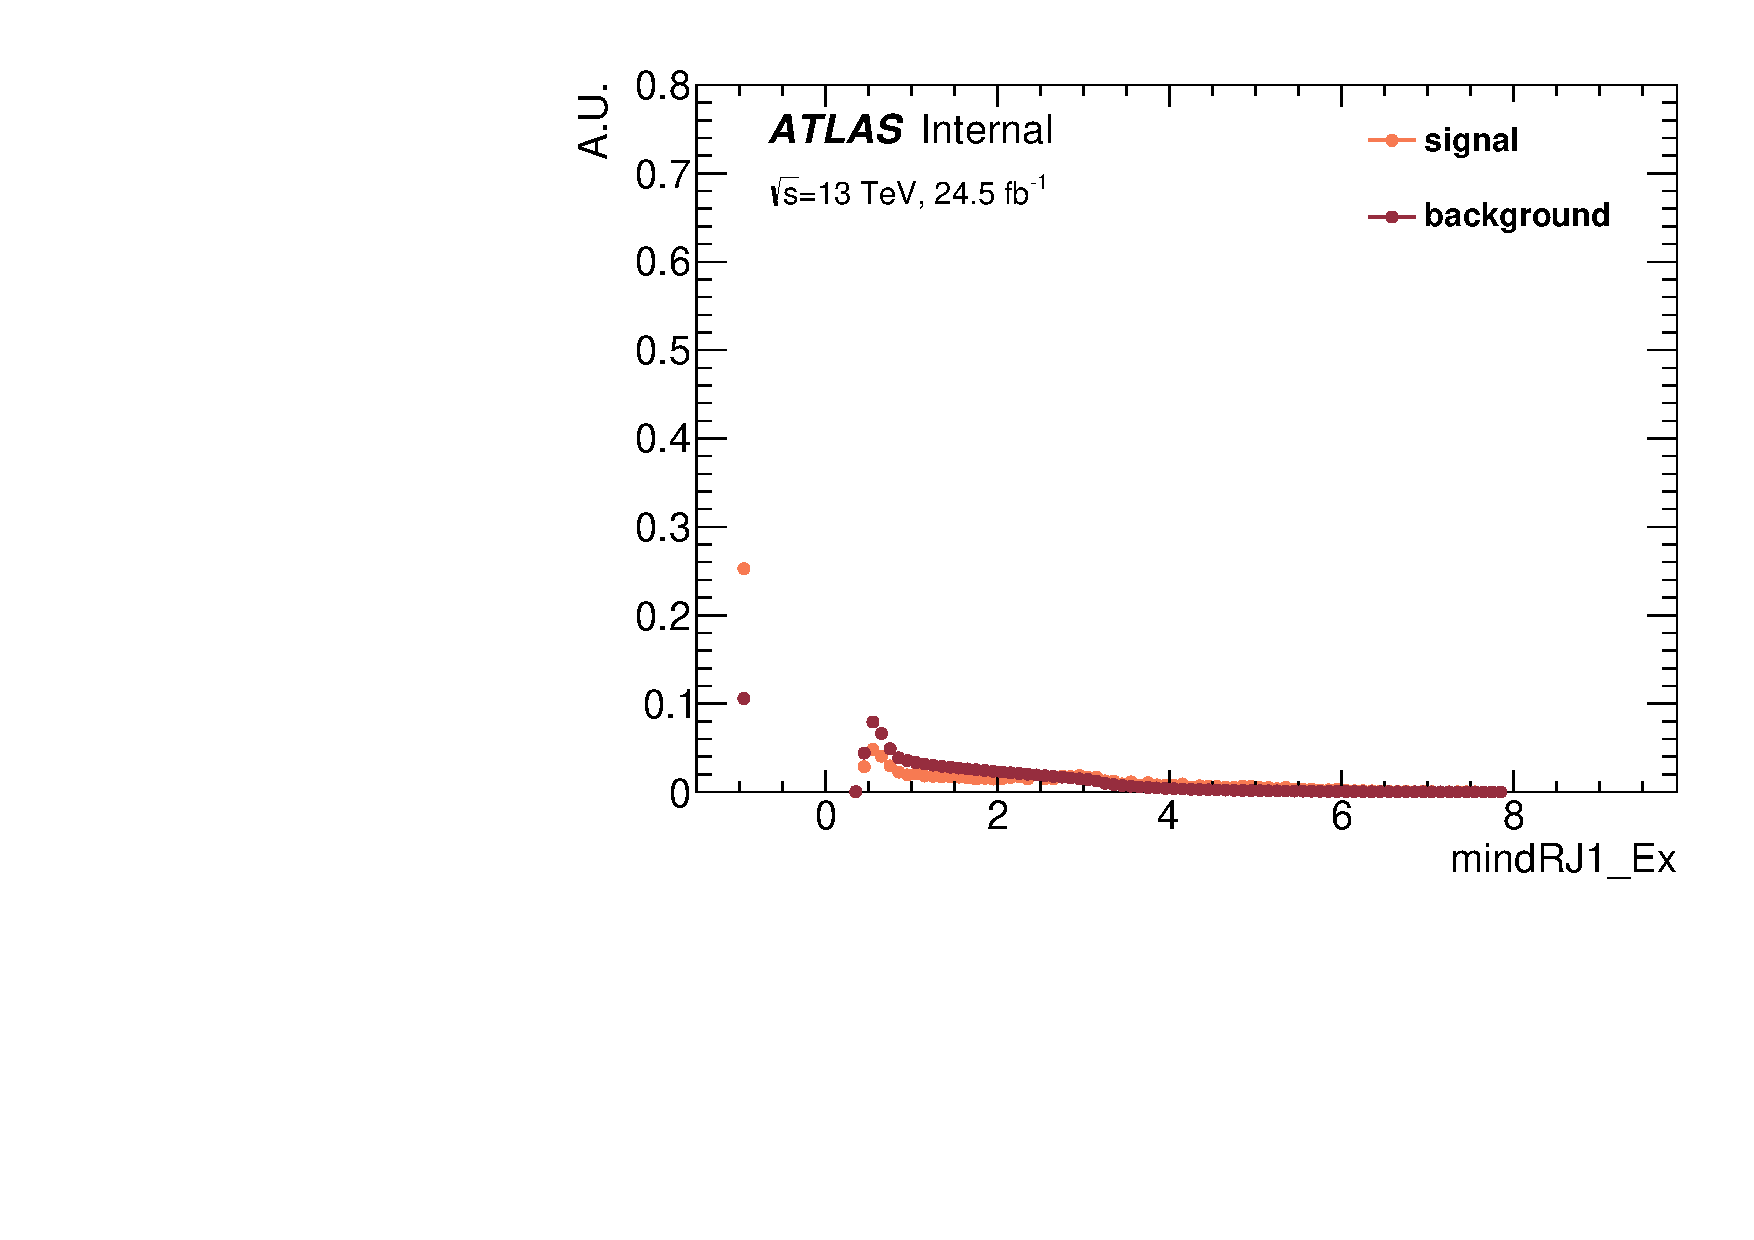
\includegraphics[width=0.3\textwidth]{figures/VBF/BDT_mindRJ1_4cen.pdf}
 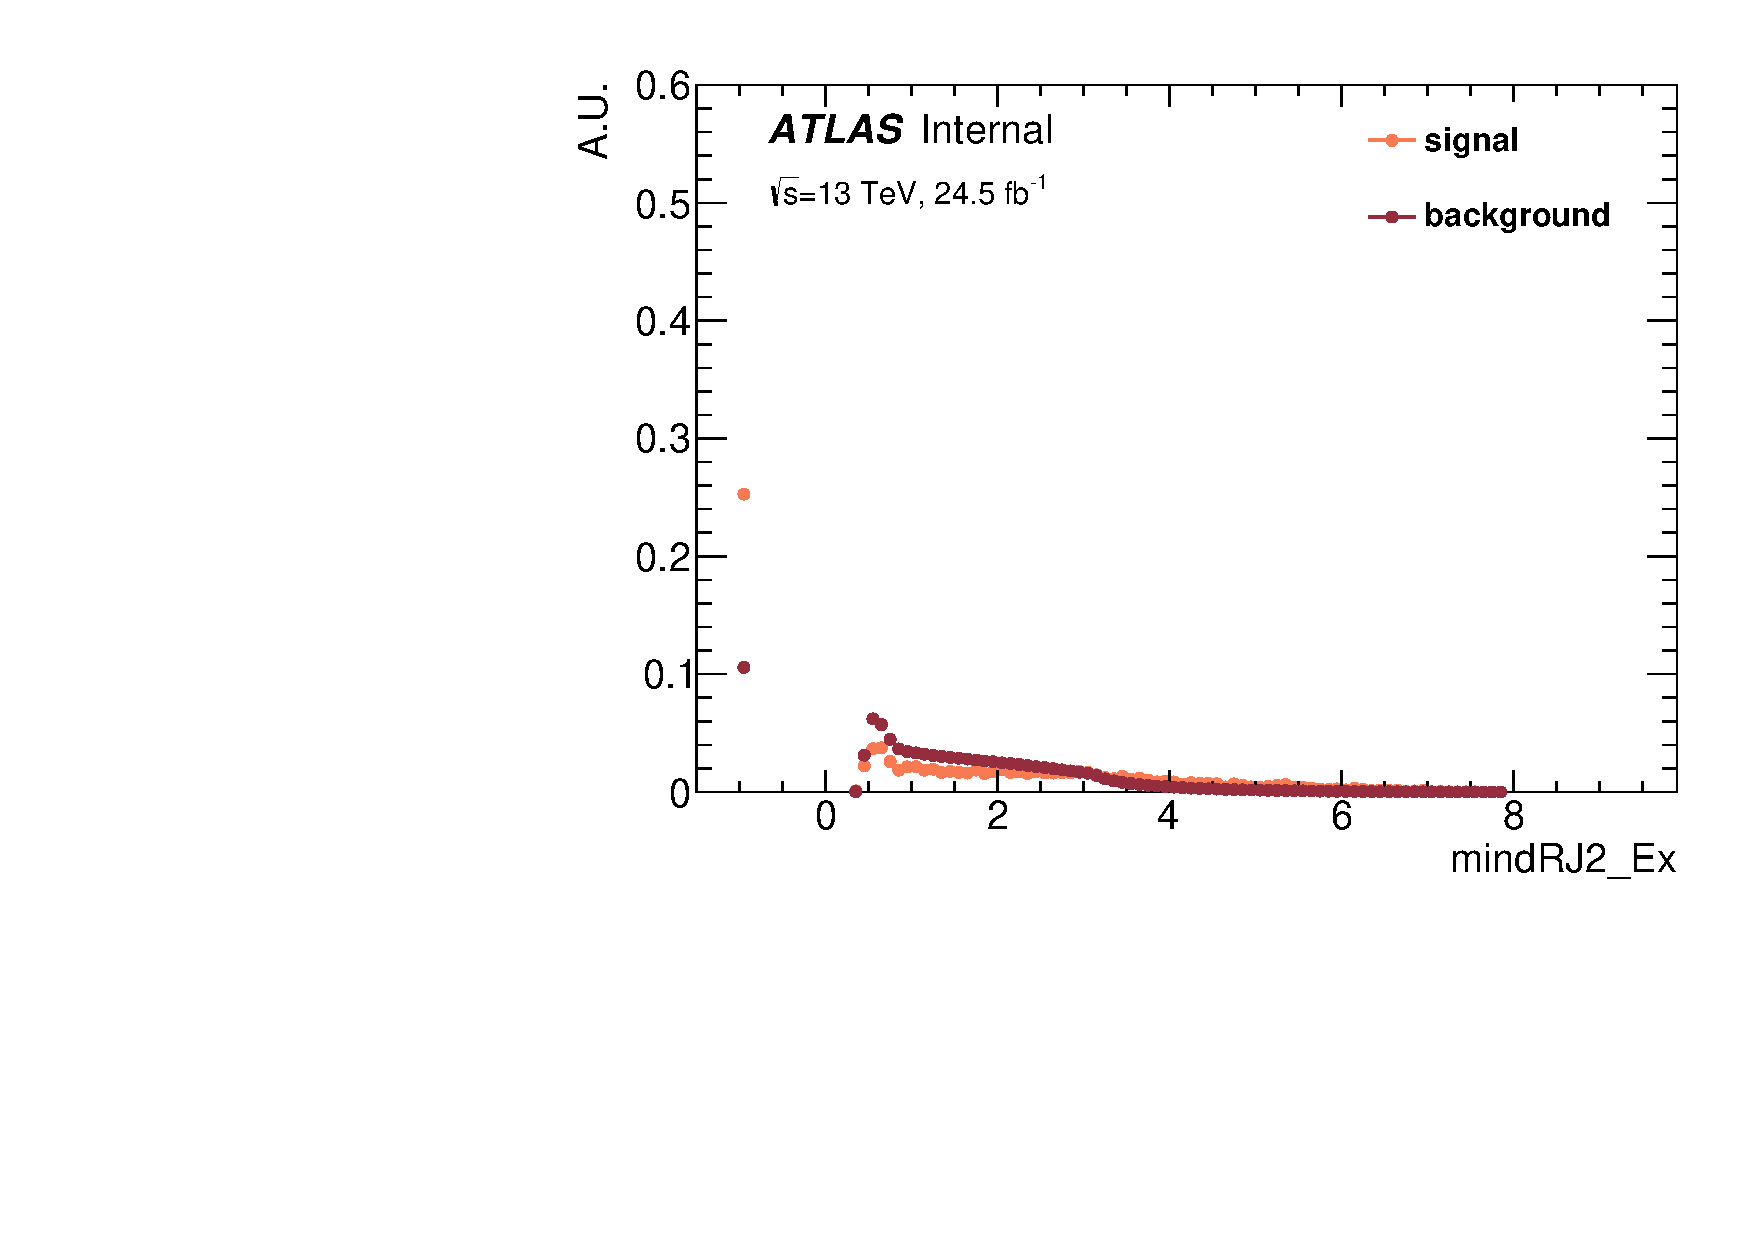
\includegraphics[width=0.3\textwidth]{figures/VBF/BDT_mindRJ2_4cen.pdf}
 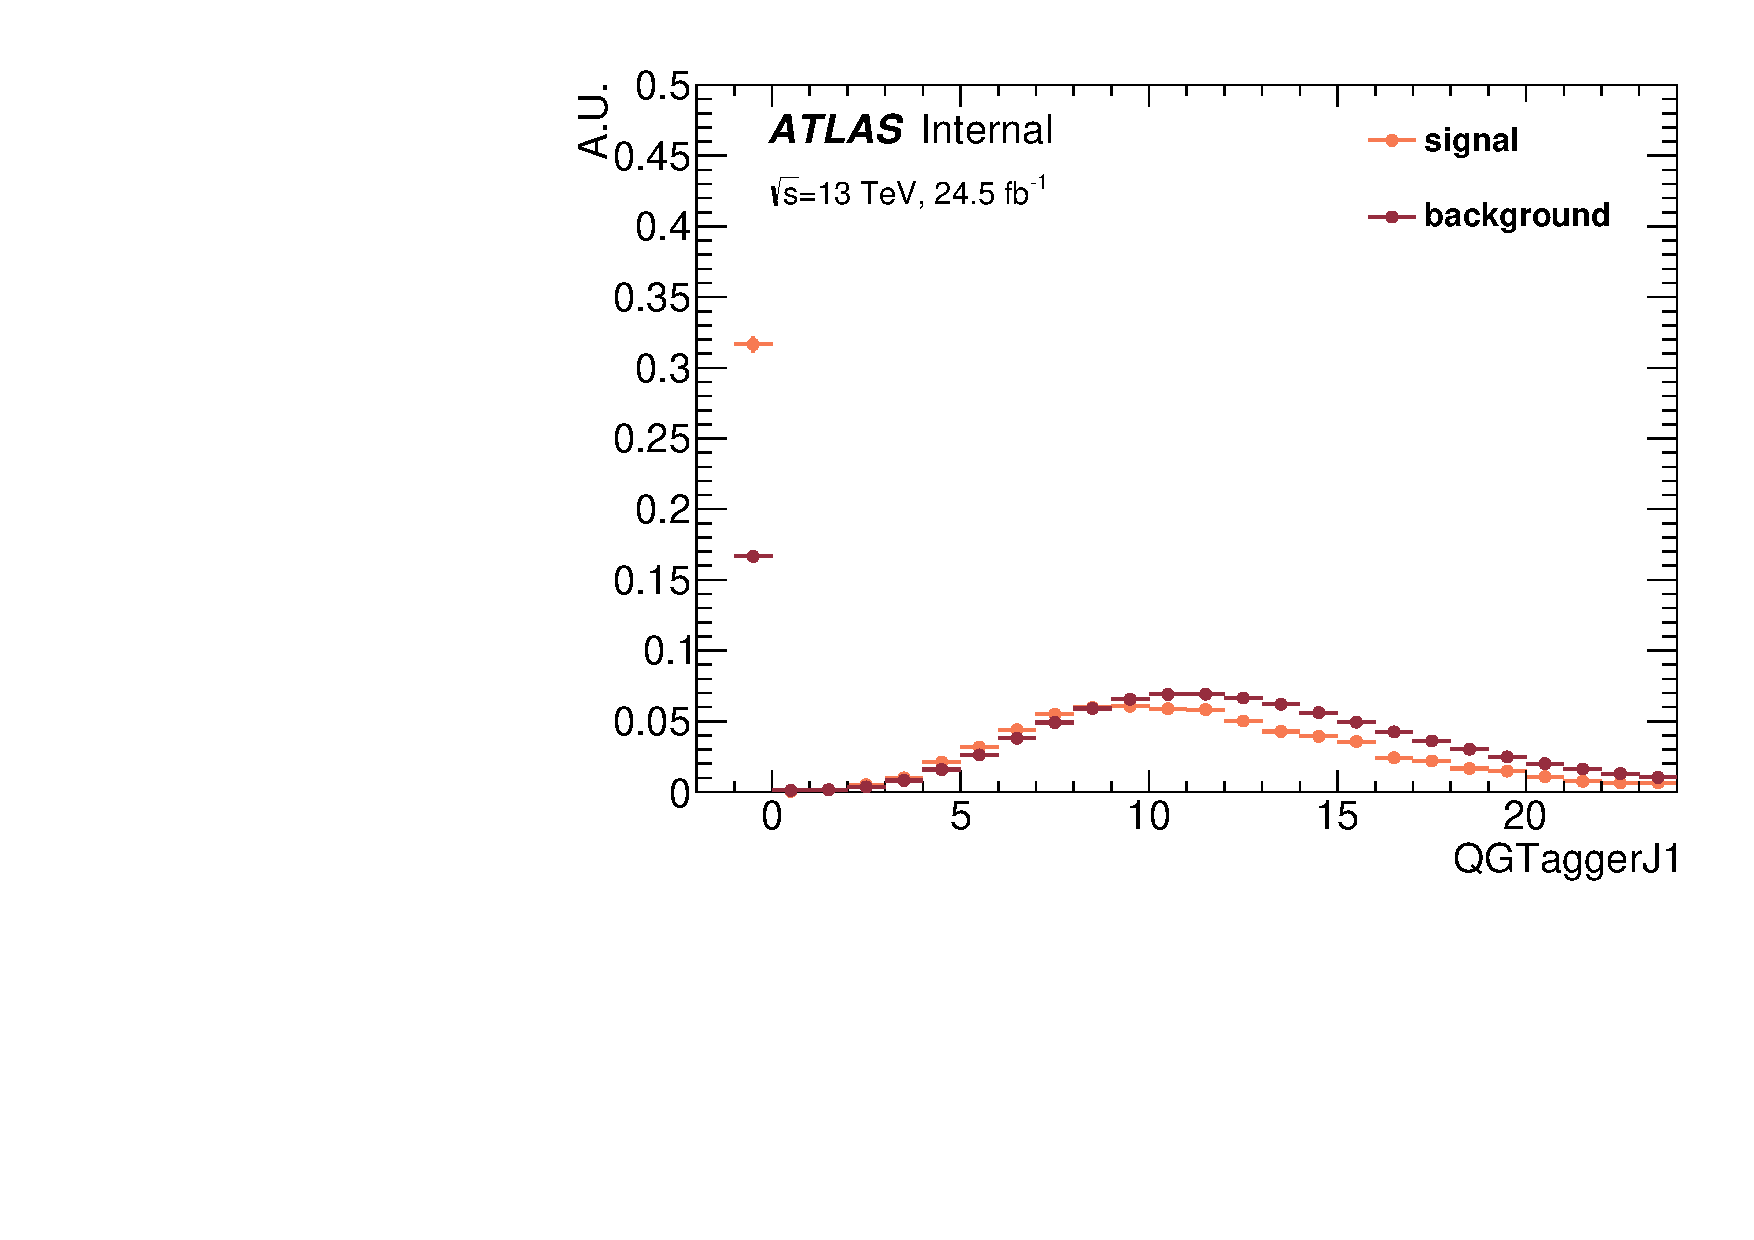
\includegraphics[width=0.3\textwidth]{figures/VBF/BDT_NTrk500_J1_4cen.pdf}\\
 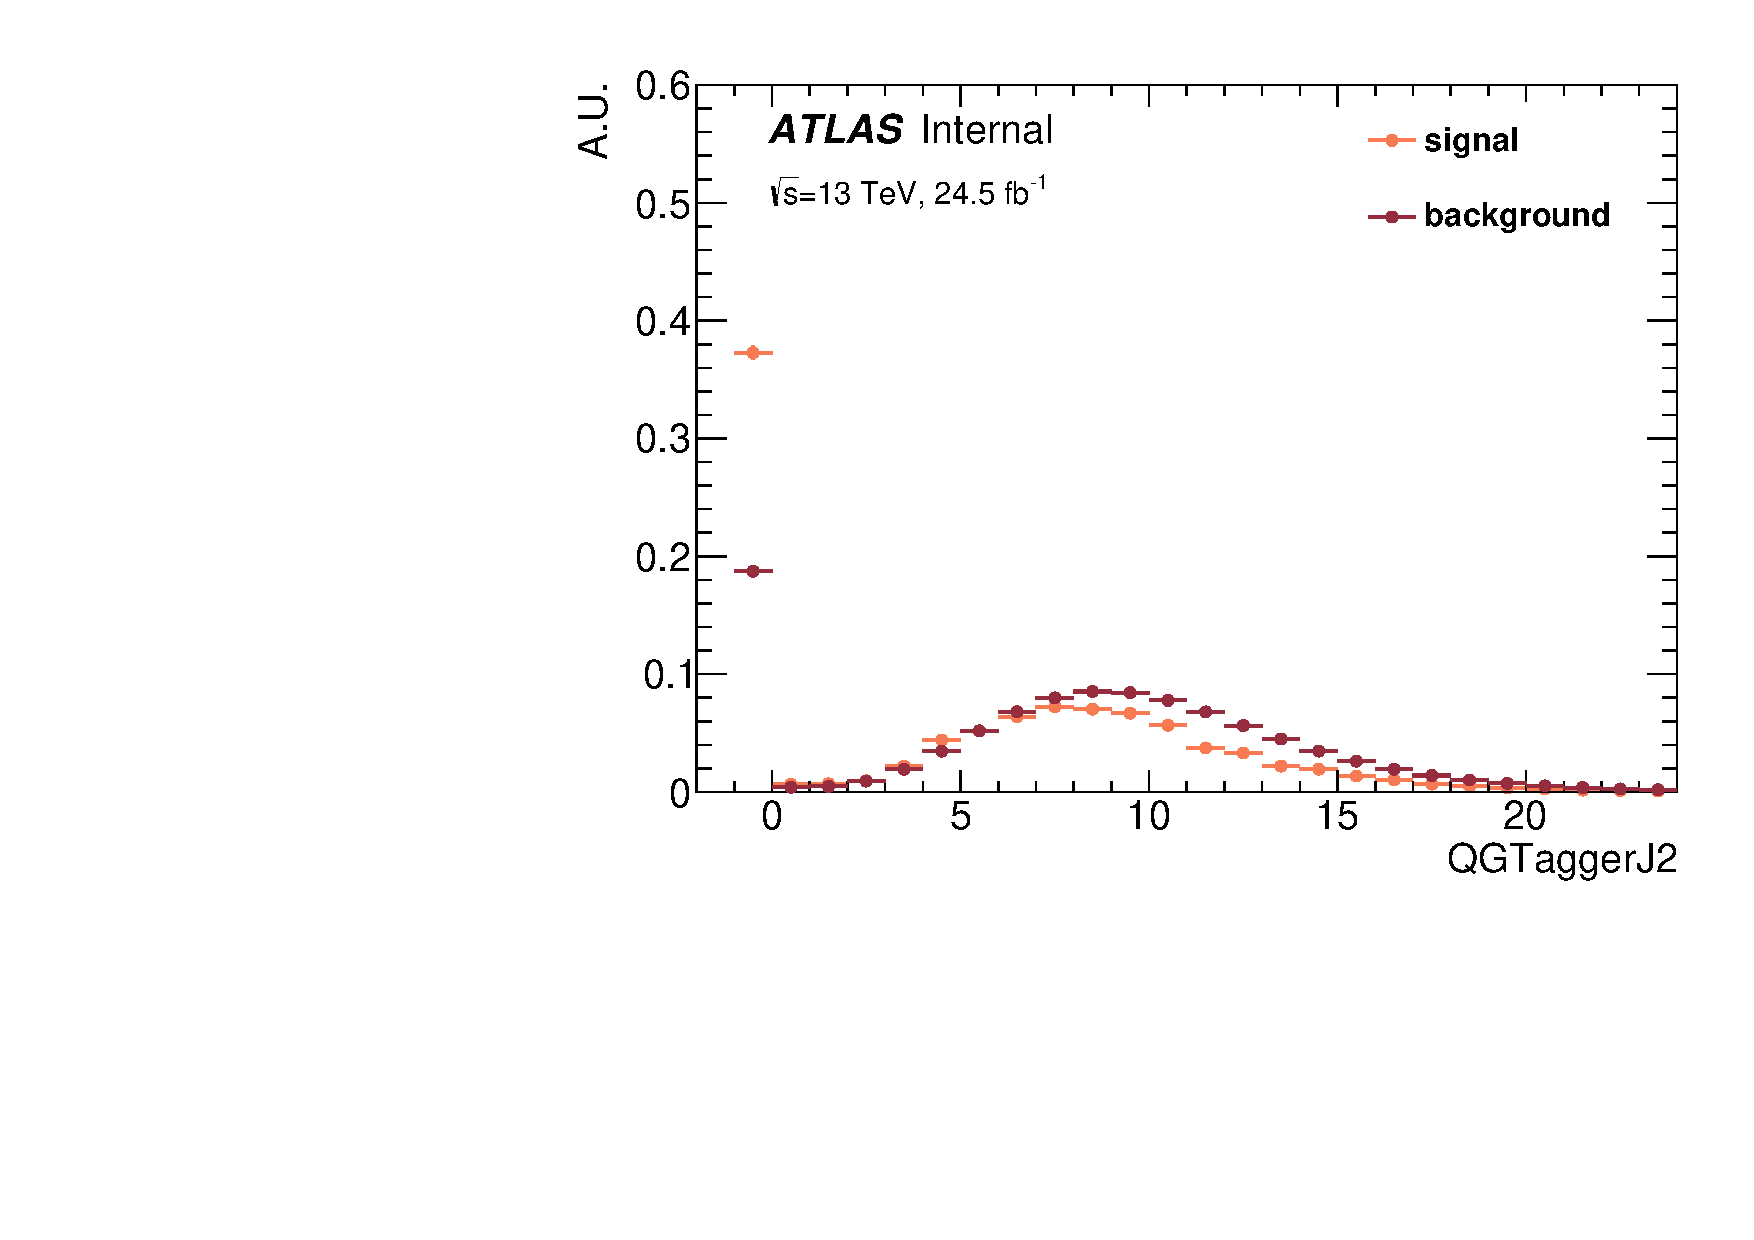
\includegraphics[width=0.3\textwidth]{figures/VBF/BDT_NTrk500_J2_4cen.pdf}
 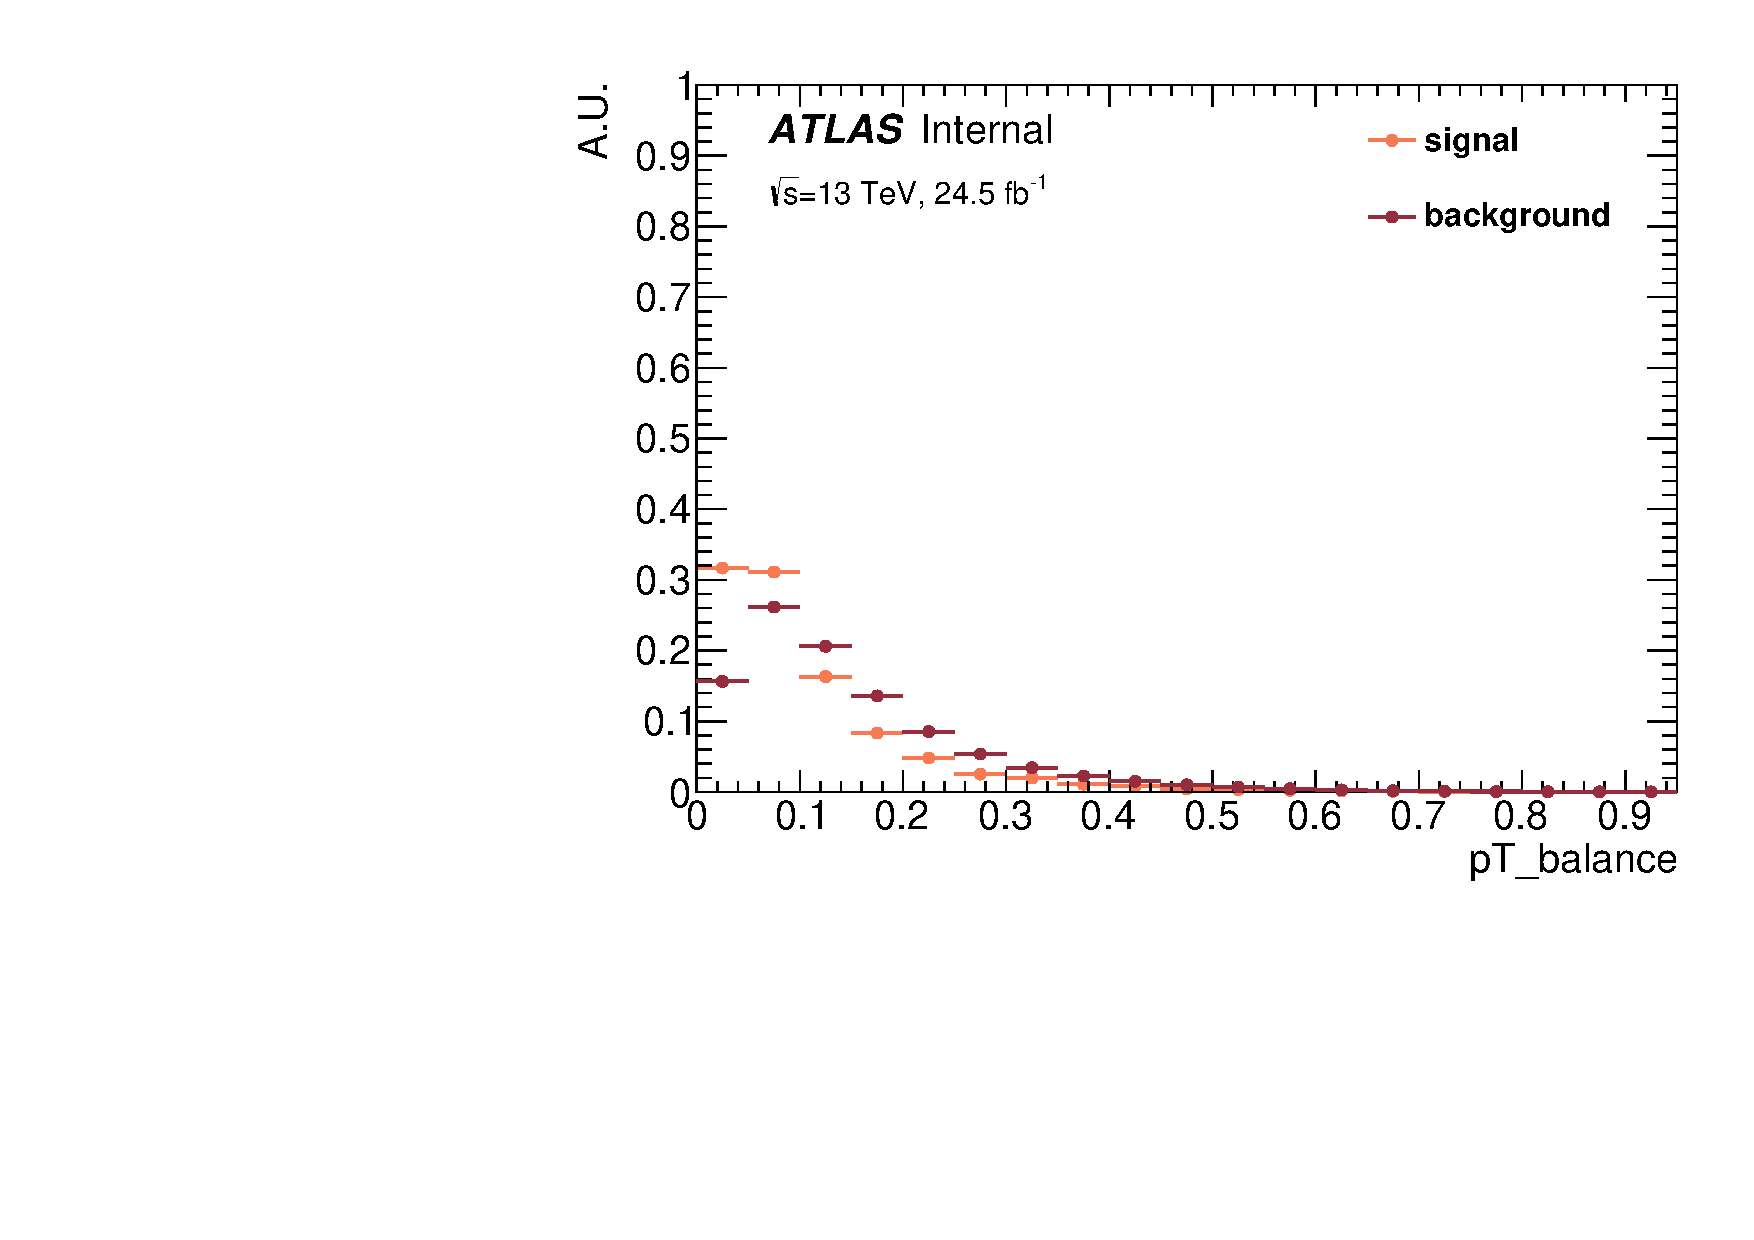
\includegraphics[width=0.3\textwidth]{figures/VBF/BDT_pTBalance_4cen.pdf}\\

\caption{Distributions of BDT input variables of \fourcentral channel}
  \label{fig:vbf-BDTInputs4cen}
\end{figure}


\begin{figure}[htbp]
  \centering
 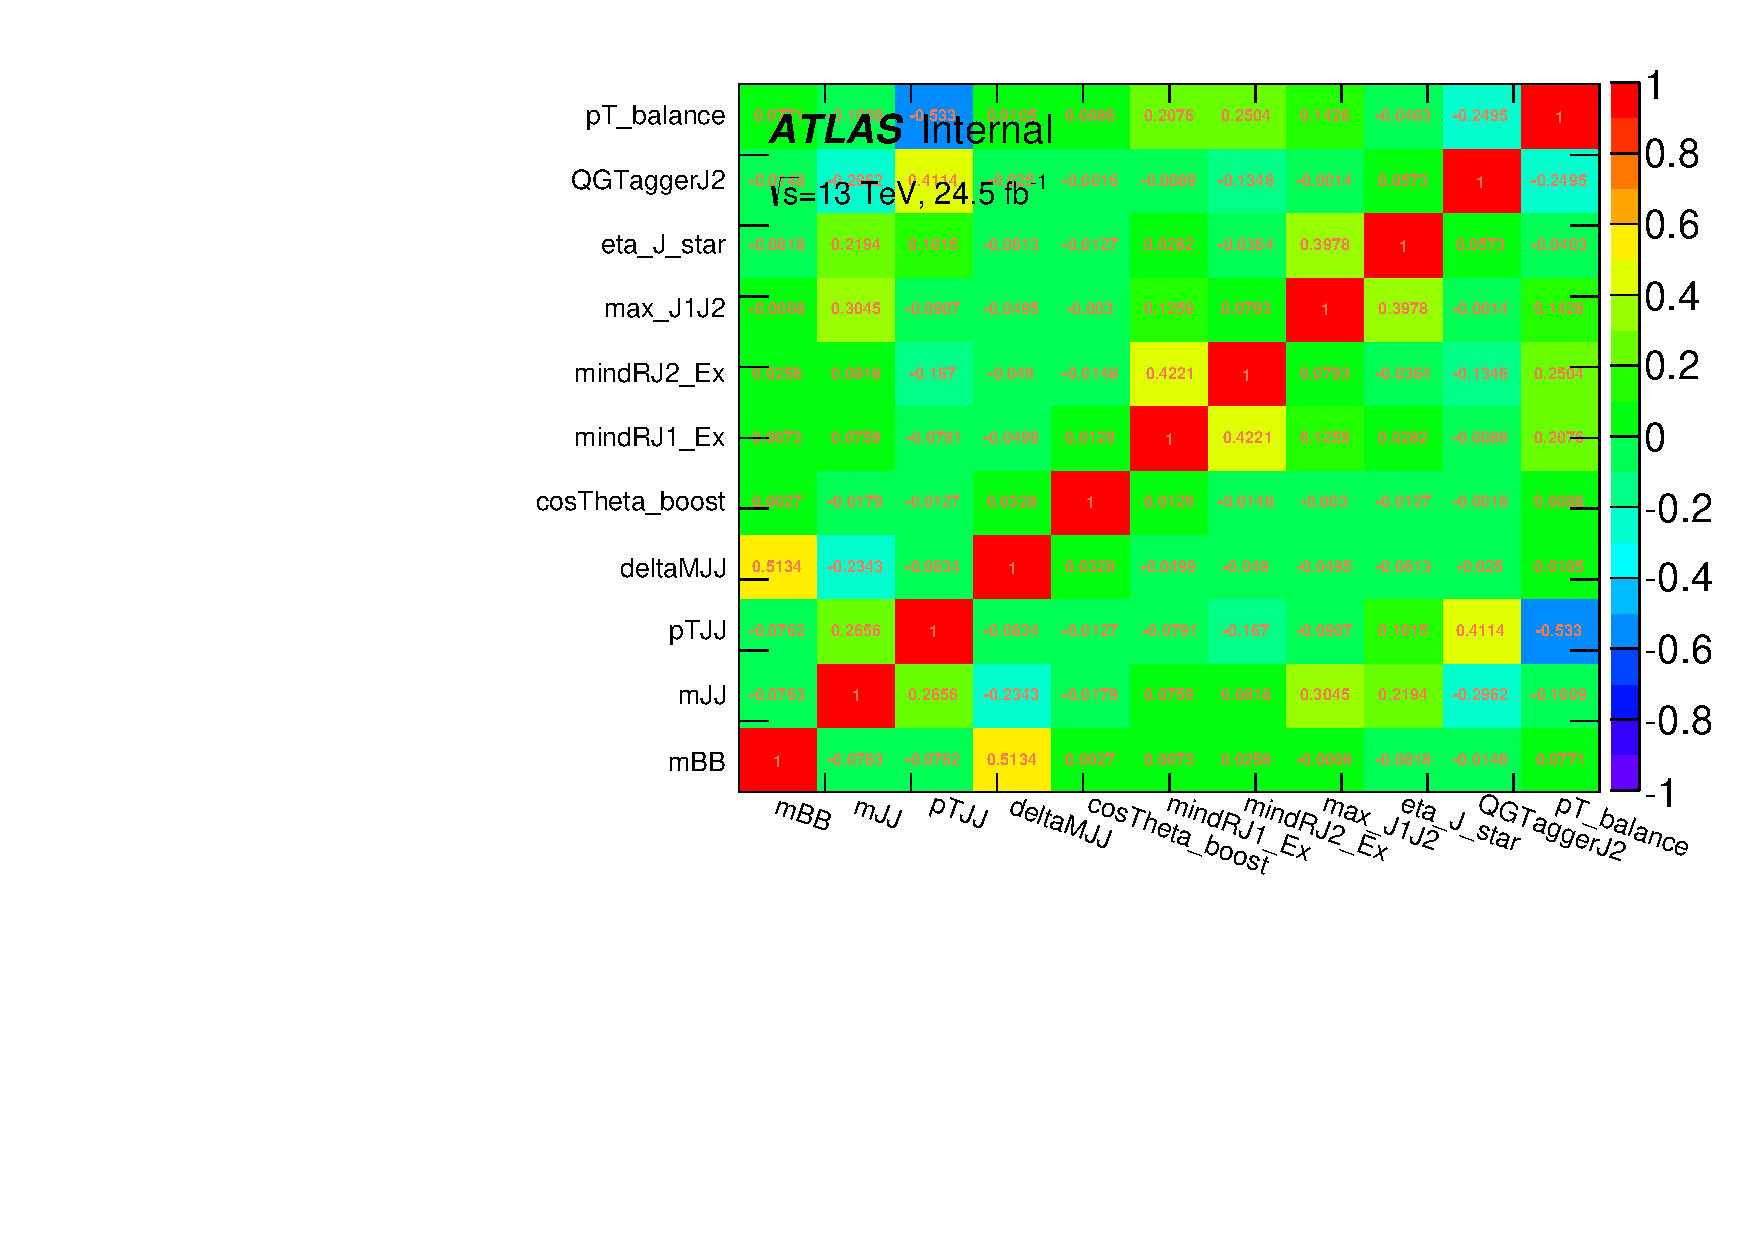
\includegraphics[width=0.48\textwidth]{figures/VBF/BDT_VBF_var_cor_2cen.pdf}
 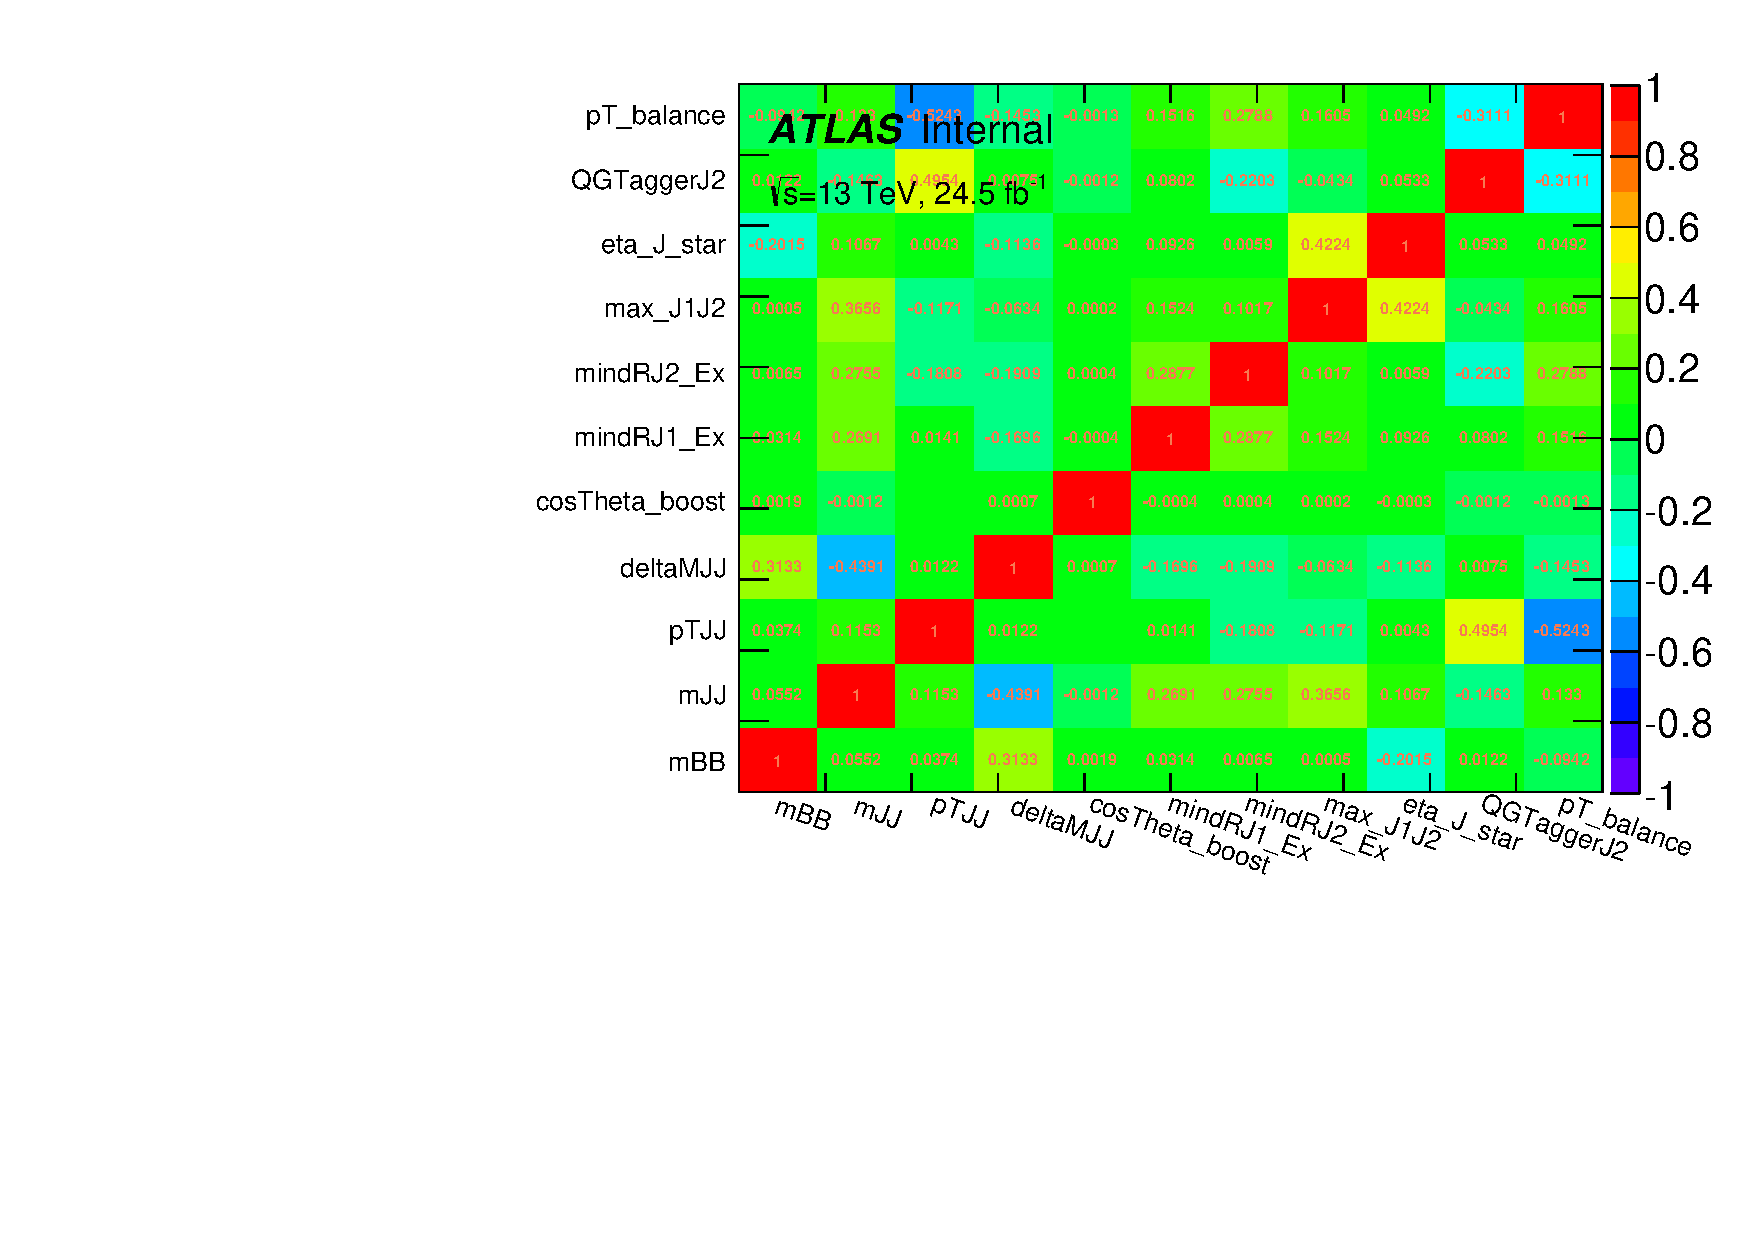
\includegraphics[width=0.48\textwidth]{figures/VBF/BDT_data_var_cor_2cen.pdf}\\
 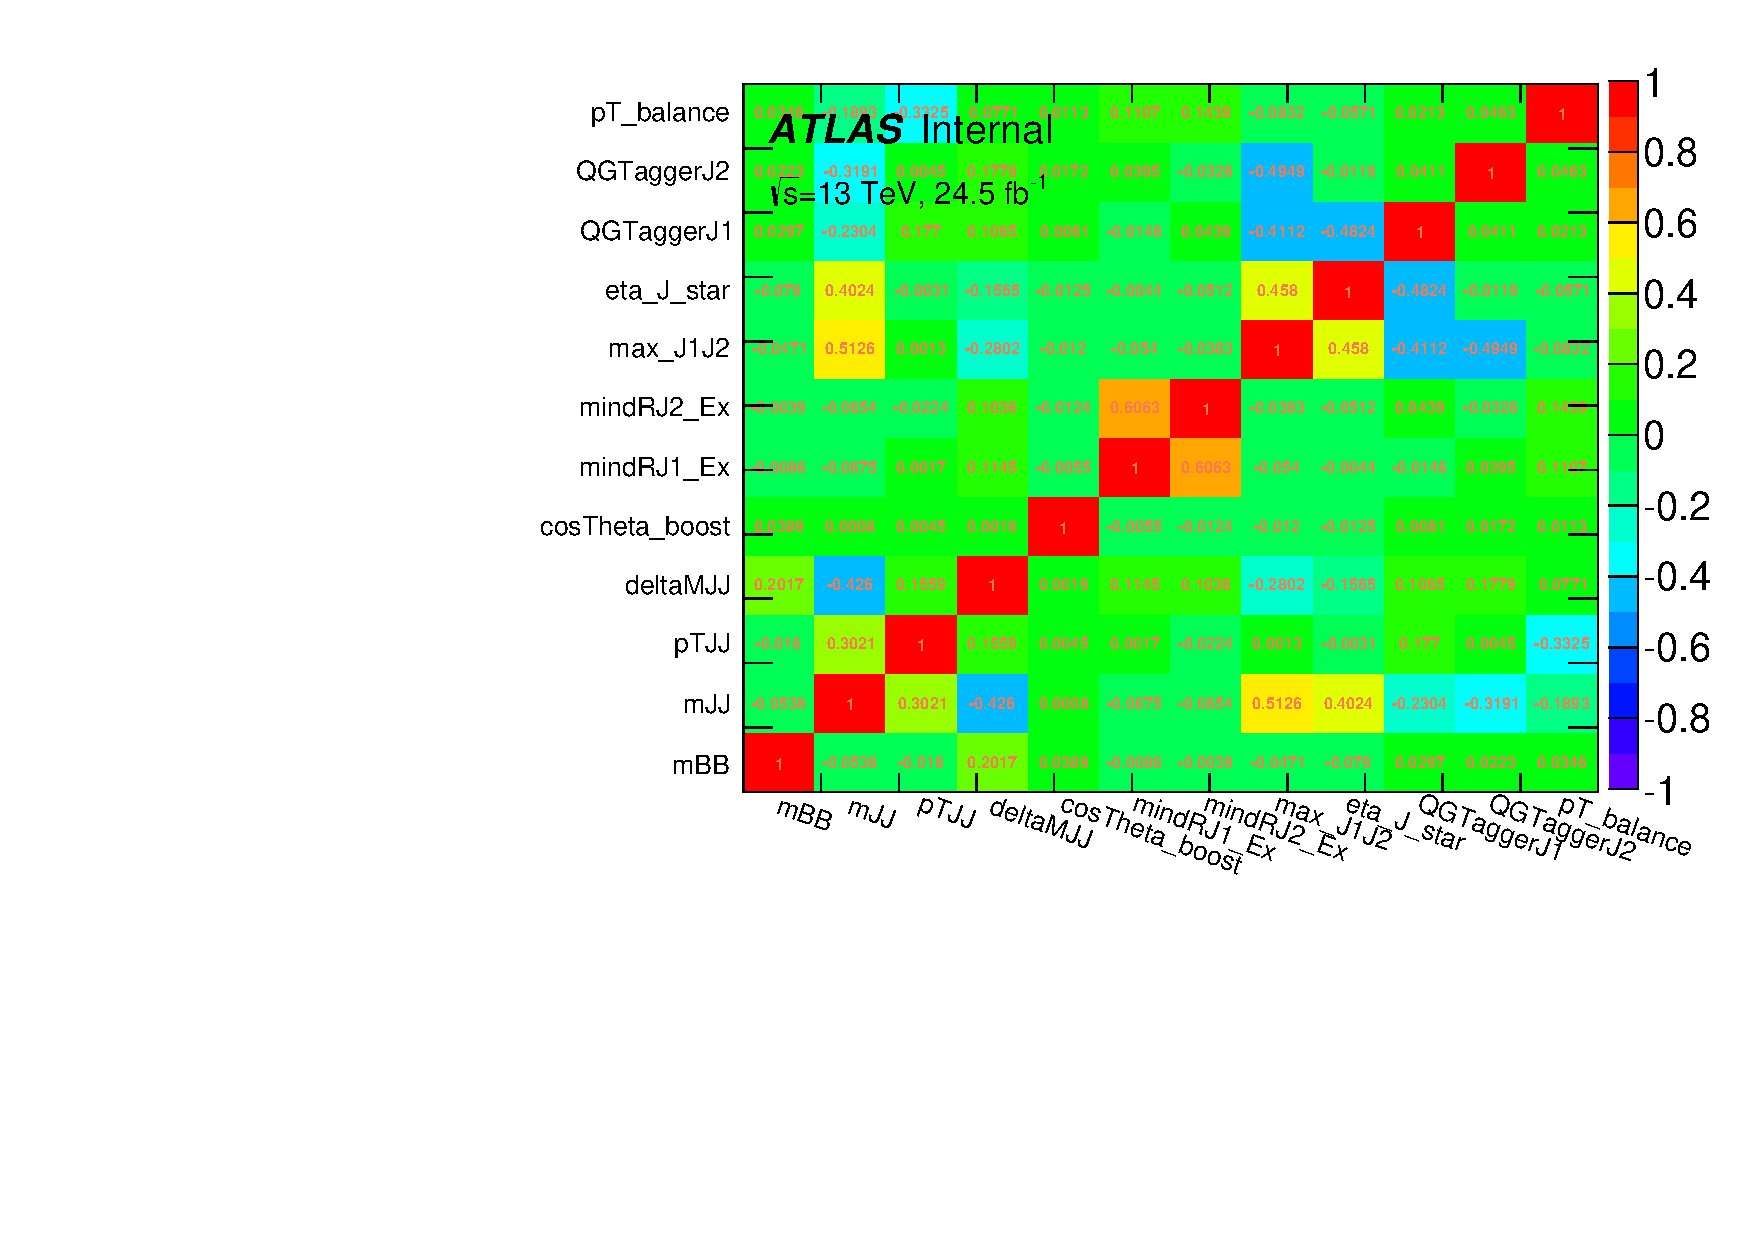
\includegraphics[width=0.48\textwidth]{figures/VBF/BDT_VBF_var_cor_4cen.pdf}
 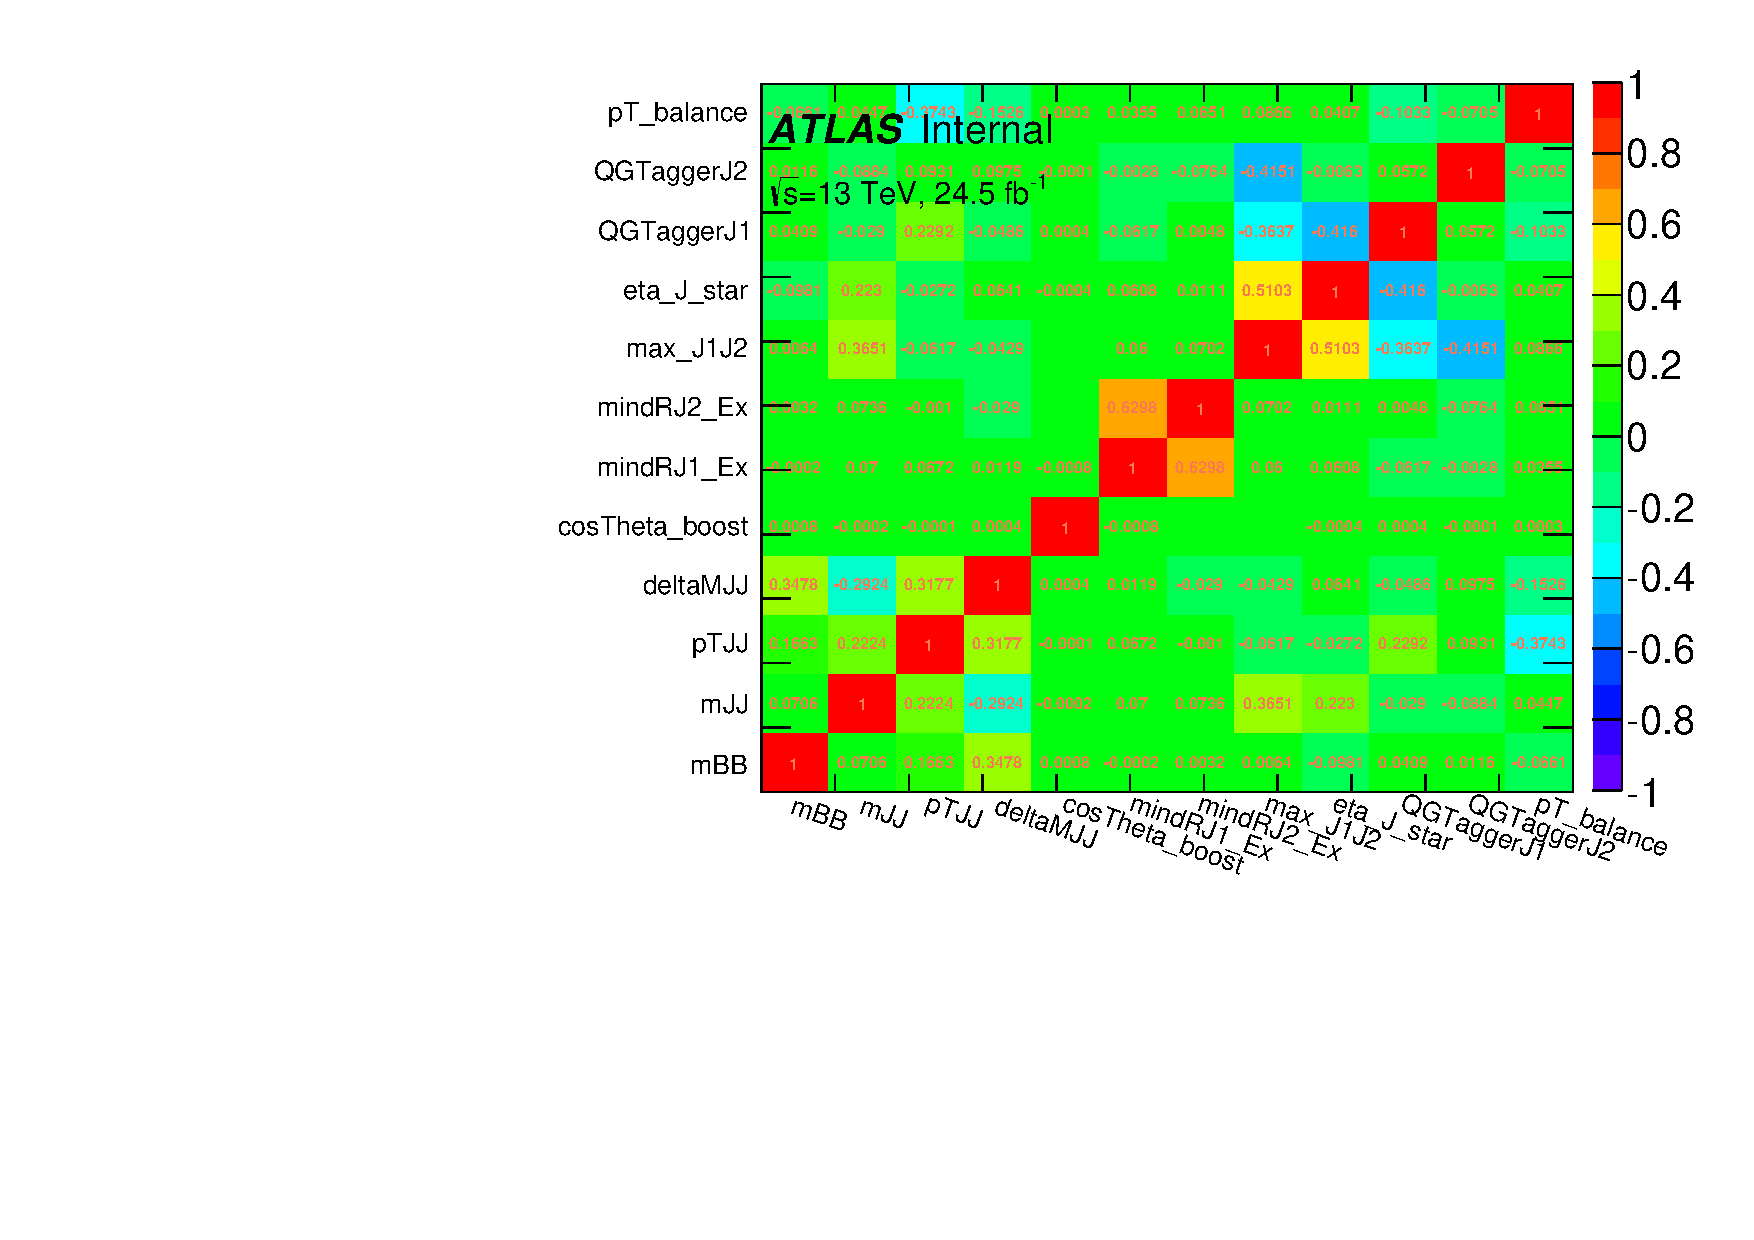
\includegraphics[width=0.48\textwidth]{figures/VBF/BDT_data_var_cor_4cen.pdf}\\
\caption{Correlations between BDT input variables and $\Mbb$ of signal (left) and background (right) of  the \twocentral (top) and \fourcentral (bottom) channels.}
  \label{fig:vbf-BDTInputsCor}
\end{figure}

\begin{figure}[htbp]
  \centering
 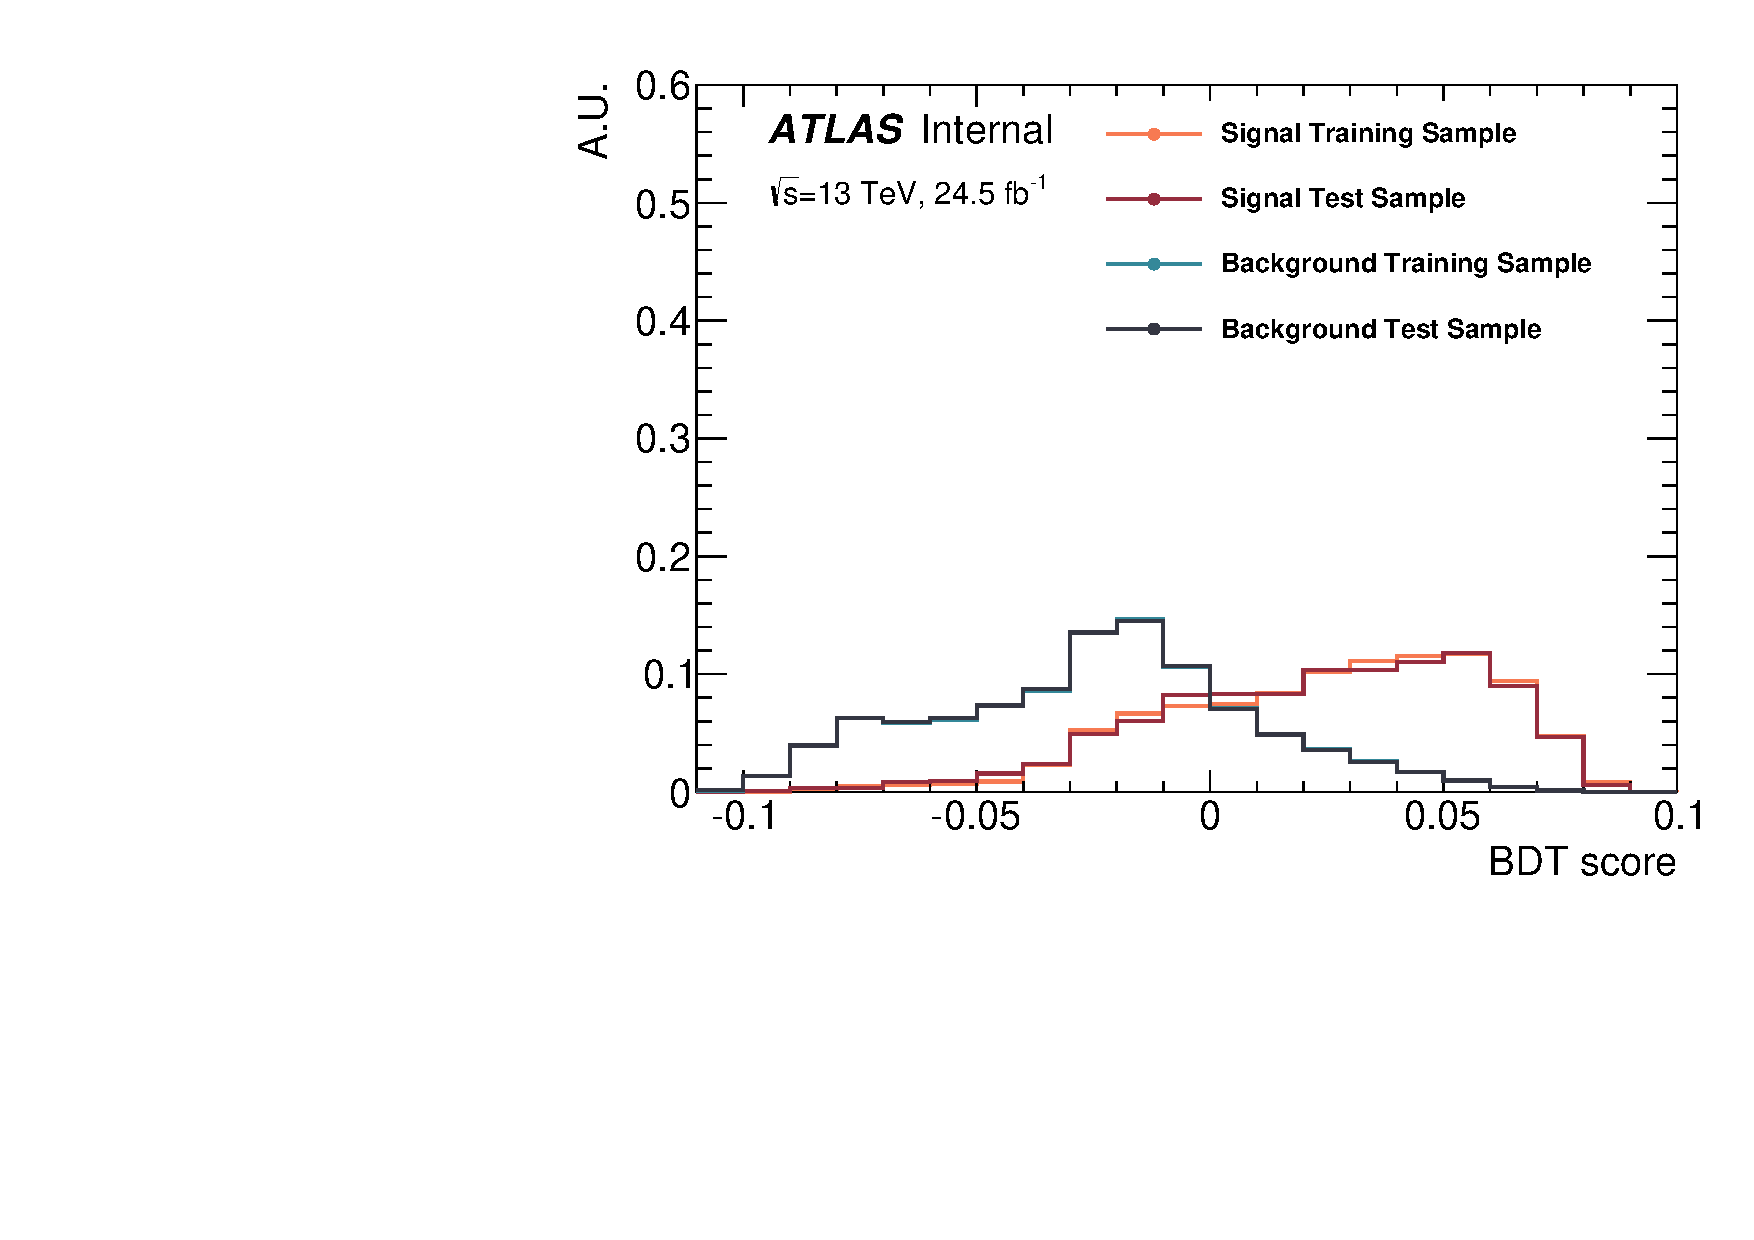
\includegraphics[width=0.48\textwidth]{figures/VBF/BDT_score_2cen.pdf}
 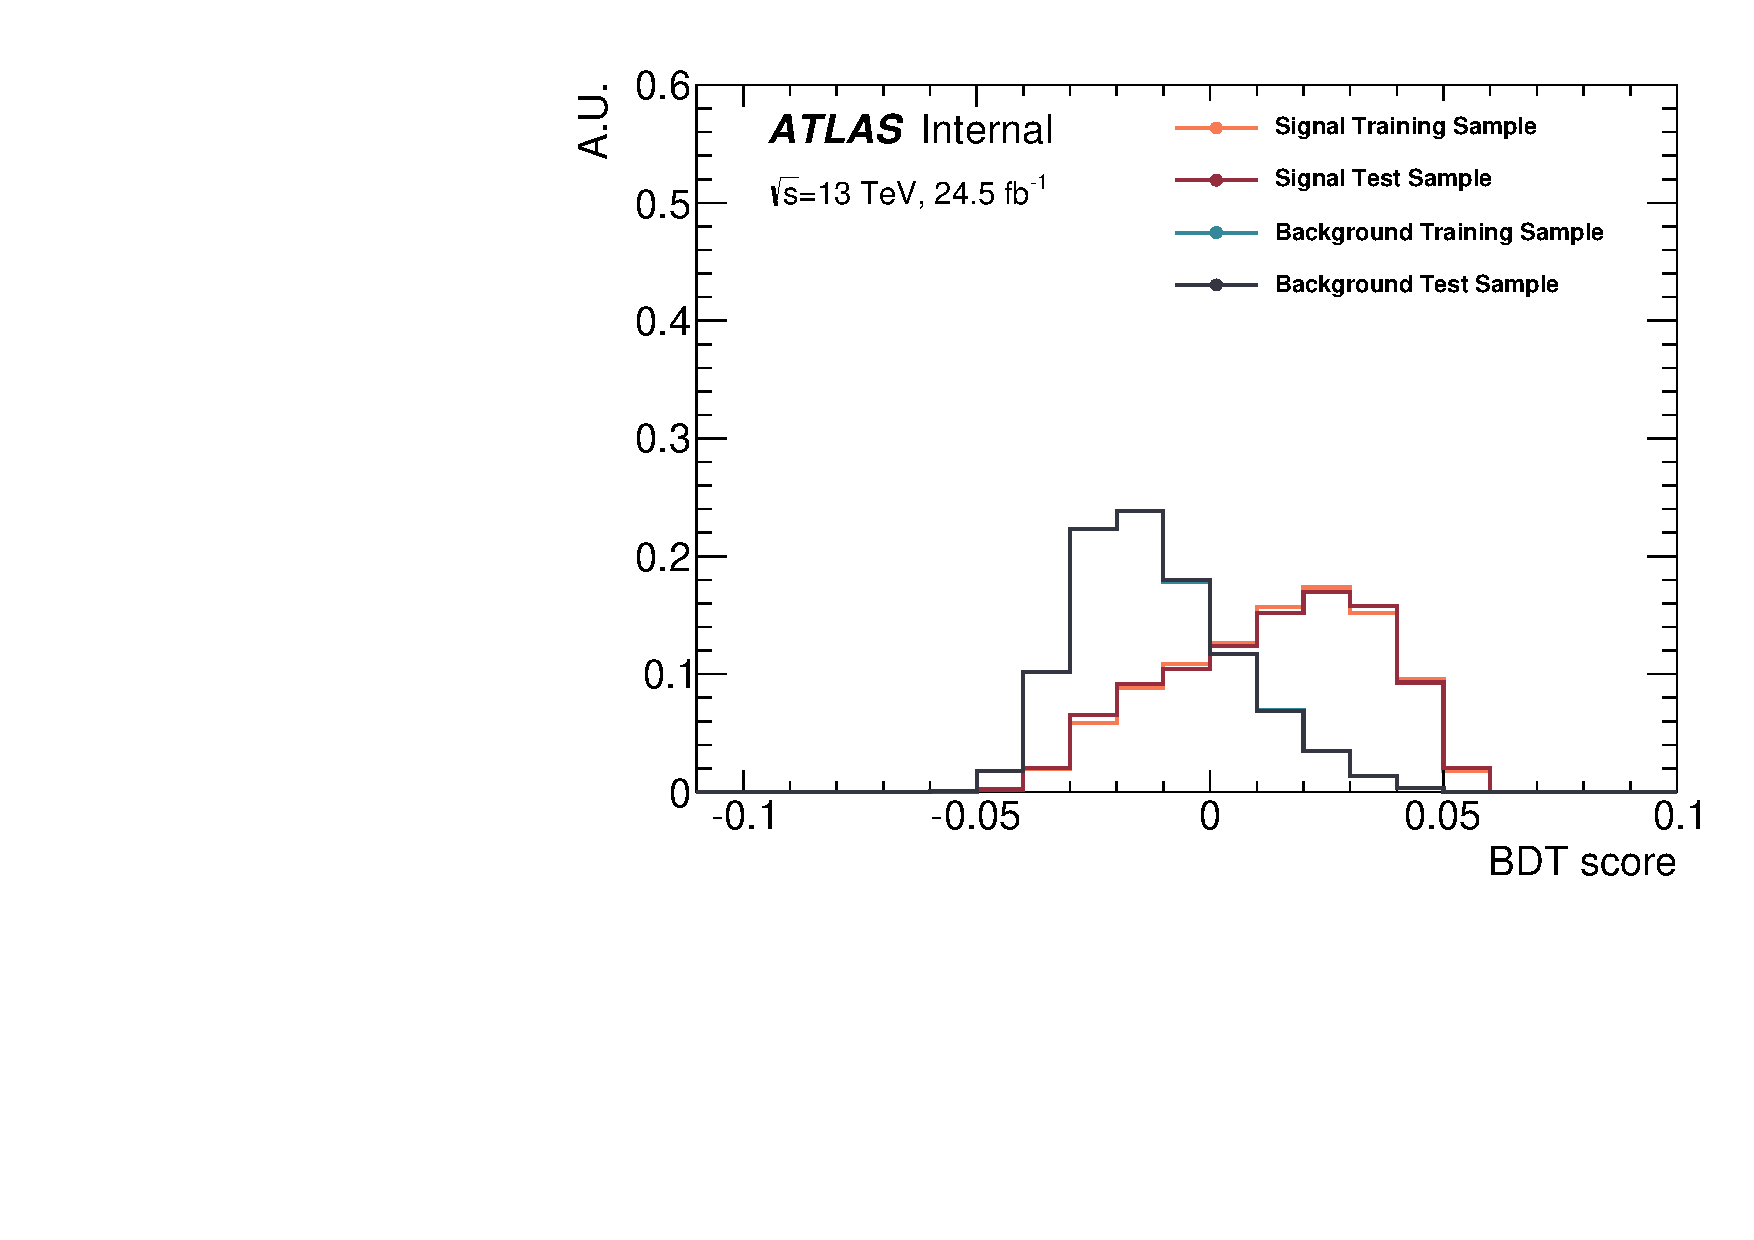
\includegraphics[width=0.48\textwidth]{figures/VBF/BDT_score_4cen.pdf}\\
 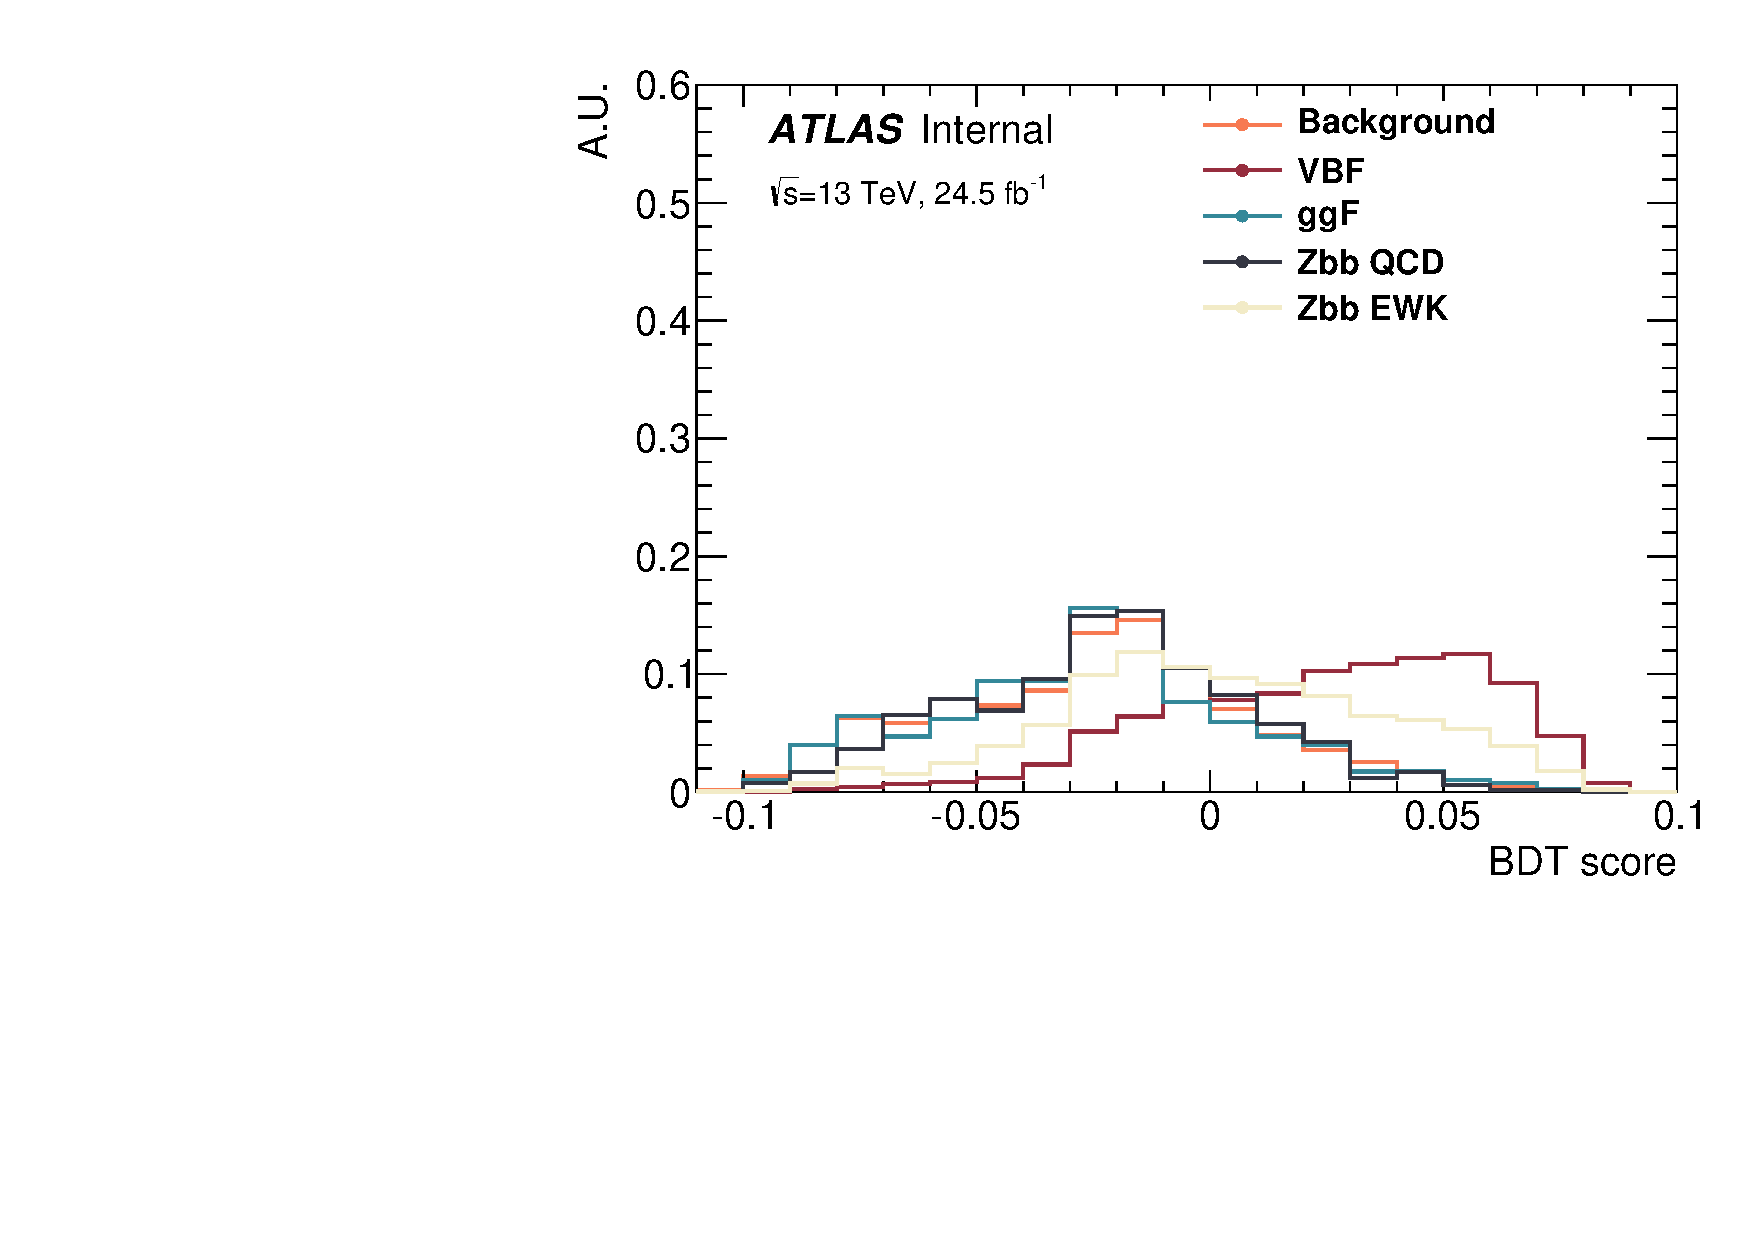
\includegraphics[width=0.48\textwidth]{figures/VBF/BDT_score_breakdown_2cen.pdf}
 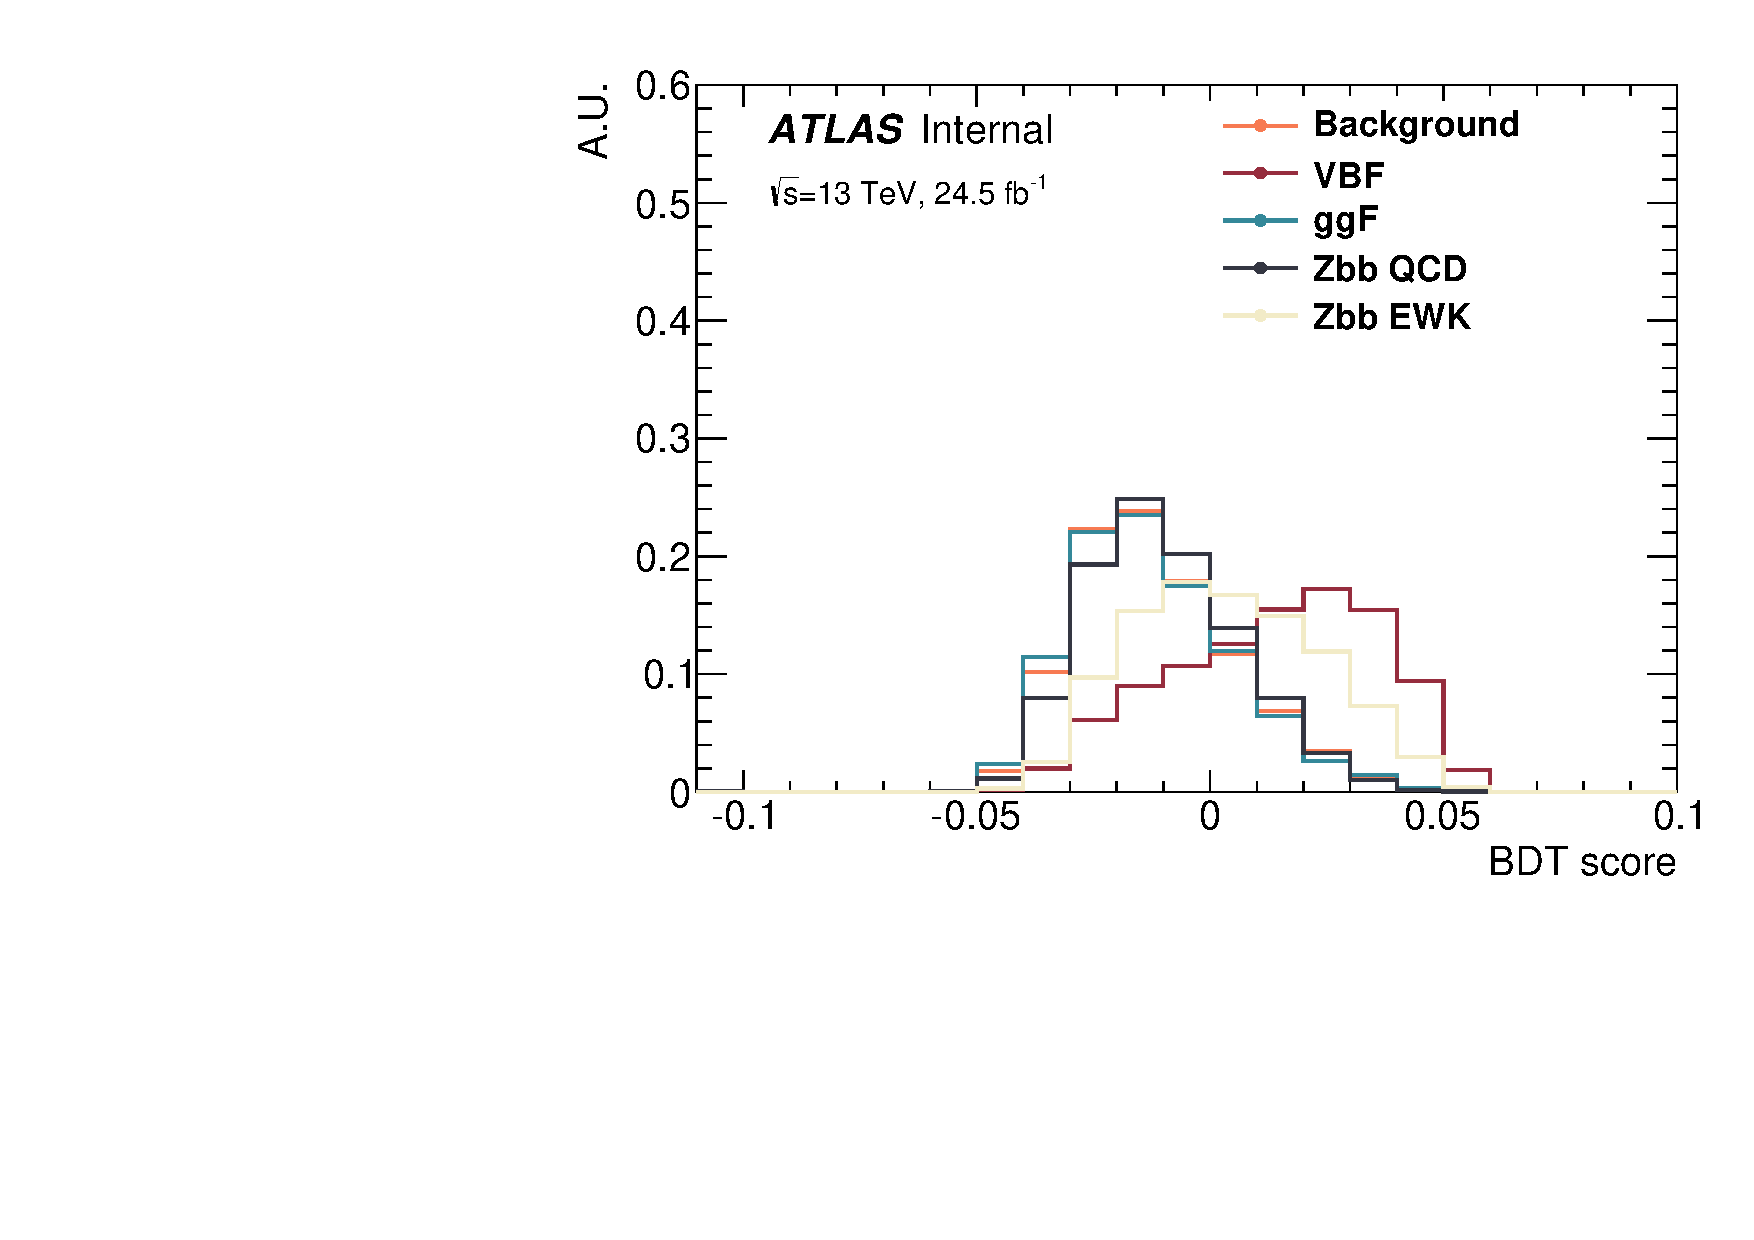
\includegraphics[width=0.48\textwidth]{figures/VBF/BDT_score_breakdown_4cen.pdf}\\
\caption{BDT Response for  the \twocentral (left) and \fourcentral (right) channel.  The top row shows the response for both the training and validation samples.  The bottom row shows a comparison of response for the signal, multijet background, $ggF$ Higgs and $Z$ boson samples. }
  \label{fig:vbf-BDTResponse}
\end{figure}


